% \tableofcontents % enable to generate .toc file used in listings.tex
\section{Introduction}\label{sec:level1}
Music is usually defined as the art whose medium is sound.
The definition might also state that the medium includes silences
and temporal organization of structures, or that music
is also a cultural activity or product.
In physics and in this document, sounds are longitudinal waves of mechanical pressure.
The human auditory system perceives sounds in the frequency bandwidth between $20Hz$ and $20kHz$,
with the actual boundaries depending on the person,
climate conditions and the sonic characteristics themselves.
Since the speed of sound is $\approx 343.2 m/s$,
such frequency limits corresponds to  wavelengths of $\frac{343.2}{20} \approx 17.16\,m$ and
$\frac{343.2}{20000} \approx 17.16\,mm$.
Hearing involves stimuli in bones, stomach, ears,
transfer functions of head and torso,
and processing by the nervous system.
The ear is a dedicated organ for the appreciation of these waves,
which decomposes them into their sinusoidal spectra and delivers to the nervous system.
The sinusoidal components are crucial to musical phenomena,
as one can recognize in the constitution of sounds of musical interest
(such as harmonic sounds and noises, discussed in Sections~\ref{sec:discNote} and~\ref{sec:internalVar}),
and higher level musical structures (such as tunings, scales and chords, in the Supporting Information document~\cite{massNotesInMusic}).~\cite{Roederer}

\begin{figure*}[!h]
    \centering
        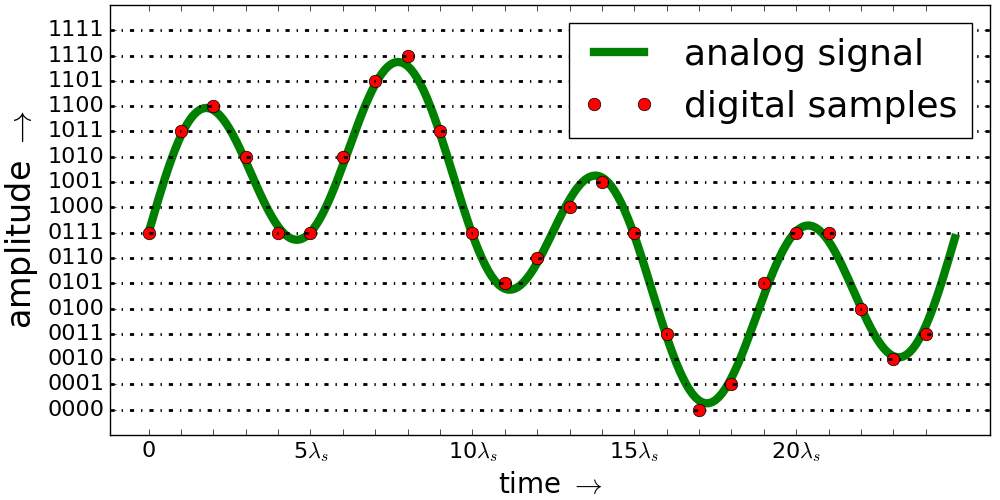
\includegraphics[width=.7\textwidth]{figures/pcm_}
	\caption{Example of PCM audio:
	a sonic wave is represented by 25 samples equally spaced in time, where each sample has an amplitude specified with 4 bits.}
        \label{fig:PCM}
\end{figure*}

The representation of sound can take many forms,
from musical scores and texts in a phonetic language to electric analog signals and binary data.
It includes sets of features such as wavelet or sinusoidal components.
Although the terms 'audio' and 'sound' are often used without distinction
and 'audio' has many definitions which depend on the context and the author,
audio most often means a representation of the amplitude through time.
In this sense,
audio expresses sonic waves yield by synthesis or input by microphones,
although these sources are not always neatly distinguishable
e.g. as captured sounds are processed to generate new sonorities.
Digital audio protocols often imply in quality loss (to achieve smaller files, ease storage and transfer)
and are called \emph{lossy}~\cite{loss}.
This is the case e.g. of MP3 and Ogg Vorbis.
Non-lossy representations of digital audio, called \emph{lossless} protocols or formats,
on the other hand, assure perfect reconstruction of the analog wave within any convenient precision.
The standard paradigm of lossless audio consists of
representing the sound with samples equally spaced
by a duration $\delta_s$, and specifying the amplitude of each sample by a fixed number of bits.
This is the linear Pulse Code Modulation (LPCM) representation of sound,
herein referred to as PCM.
A PCM audio format has two essential attributes:
a sampling frequency $f_s=\frac{1}{\delta_s}$ (also called e.g. sampling rate or sample rate),
which is the number of samples used for representing a second of sound;
and a bit depth, which is the number of bits used for specifying the amplitude of each sample.
Figure~\ref{fig:PCM} shows $25$ samples of a PCM audio with a bit depth of $4$,
which enables $2^4=16$ possible values for the amplitude of each sample
and a total of $4 \times 25= 100$ bits for representing the whole sound.

The fixed sampling frequency and bit depth
yield the quantization error or quantization noise.
This noise diminishes as the bit depth increases
while greater sampling frequency allows higher frequencies to be represented.
The Nyquist theorem asserts that the sampling frequency
is twice the maximum frequency that the represented signal can contain~\cite{Openheim}.
Thus, for general musical purposes, it is suitable to use a sample rate of
at least twice the highest frequency heard by humans,
that is, $f_s \geq 2\times 20kHz = 40kHz$.
This is the basic reason for the adoption of sampling frequencies
such as $44.1kHz$ and $48kHz$,
which are standards in Compact Disks (CD)
and broadcast systems (radio and television), respectively.

Within this framework for representing sounds,
musical notes can be characterized.
The note often stands as the 'fundamental unit' of musical structures
(such as atoms in matter or cells in macroscopic organisms) and,
in practice, it can unfold into sounds that uphold other approaches to music.
This is of capital importance because science and scholastic artists
widened the traditional comprehension of music in the twentieth century
to encompass discourse without explicit rhythm, melody or harmony.
This is evident e.g. in the concrete, electronic, electroacoustic,
and spectral musical styles.
In the 1990s, it became evident that popular
(commercial) music had also incorporated
sound amalgams and abstract discursive arcs\footnote{There
are well known incidences of such characteristics in ethnic music,
such as in Pygmy music, but western theory assimilated them
only in the last century~\cite{Wisnick}.}.
Notes are also convenient for another reason:
the average listener -- and a considerable part of the specialists --
presupposes rhythmic and pitch organization 
(made explicit in the Supporting Information document~\cite{massNotesInMusic})
as fundamental musical properties,
and these are developed in traditional musical theory in terms of notes.
Thereafter, in this article we describe musical notes in PCM audio through equations
and then indicate mechanisms for deriving higher level musical structures.
We understand that this is not the unique approach to mathematically express music in
digital audio, but musical theory and practice suggest that
this is a proper framework for understanding and making computer music,
as should become patent in the reminder of this text and is verifiable
by usage of the \massa\ toolbox.
Hopefully, the interested reader or programmer will be able to use
this framework to synthesize music beyond traditional conceptualizations when intended.

% \subsection{Contributions and paper organization}
This document provides a
fundamental description of musical structures
in discrete-time audio.
The results include mathematical relations,
usually in terms of musical characteristics and PCM samples,
concise musical theory considerations,
and their implementation as software routines both as
very raw and straightforward algorithms and in the context of rendering musical pieces.
Despite the general interests involved,
there are only a few books and computer implementations that tackle the subject directly.
These mainly focus on computer implementations and ways to mimic traditional instruments,
with scattered mathematical formalisms for the basic notions.
Articles on the topic appear to be lacking, to the best of our knowledge,
which contrasts with the advanced and specialized developments often reported.
A compilation of such works and their contributions is in the Appendix G of~\cite{dissertacao}.
Although current music software uses the analytical descriptions presented here,
there is no concise mathematical description of them, and it is far from trivial
to achieve the equations by analyzing the available software implementations.

Accordingly, the objectives of this paper are to:
\begin{enumerate}
	\item Present a concise set of mathematical and algorithmic relations between basic musical elements and sequences of PCM audio samples.
	\item Introduce a framework for sound and musical synthesis with control at sample level which entails potential uses in psychoacoustic experiments, data sonification and synthesis with extreme precision (recap in Section~\ref{cap:conclusao}).
	\item Provide a powerful theoretical framework which can be used to synthesize musical pieces and albums.
	\item Provide approachability to the developed framework\footnote{All
		the analytic relations presented in this article are implemented as small scripts in public domain.
		They constitute the \massa\ toolbox, available in an open source Git repository~\cite{gitBook}.
		These routines are written in Python and make use of Numpy,
		which performs numerical routines efficiently (e.g. through LAPACK),
		but the language and packages are by no means mandatory.
		Part of the scripts has been ported to JavaScript
		(which favors their use in Web browsers such as Firefox and Chromium)
		and native Python~\cite{numpy, tutpython, python}.
		These are all open technologies, published using licenses 
		that grant permission for copying,
		distributing, modifying and usage in research, development, art and education.
		Hence, the work presented here aims at being compliant with recommended
		practices for availability and validation
		and should ease co-authorship processes~\cite{Raymond,Lessig}.}.
	\item Provide a didactic presentation of the content, which is highly multidisciplinary,
		involving signal processing, music, psychoacoustics and programming.
\end{enumerate}

The reminder of this article is organized as follows:
Section~\ref{sec:discNote} characterizes the basic musical note;
Section~\ref{sec:internalVar} develops internal dynamics of musical notes;
the Supporting Information document~\cite{massNotesInMusic} tackles the organization of musical notes into
higher level musical structures~\cite{Wisnick,Webern,Lerdahl,Cook,Lacerda,Zamacois,Schoenberg,microsound}.
As these descriptions require knowledge on topics such as psychoacoustics, cultural traditions,
and mathematical formalisms, the text points to external complements as needed
and presents methods, results and discussions altogether.
Section~\ref{cap:conclusao} is dedicated to final considerations and further work.

\subsection{Additional material}
The main Supporting information document holds an extension of this article to encompass canonical music theory in order to bridge between the synthesis of notes and their organization as music~\cite{massNotesInMusic}.
Another Supporting Information document~\cite{massSampled} is dedicated to describing the sinusoidal spectra of samples sounds and illustrates using figures and the traditional wavefoms given in Section~\ref{sec:timbre}.
The third Supporting Information document~\cite{massListings}
holds commented listings of all the equations, figures, tables and sections in this document
and the scripts in the \massa\ toolbox.
The last Supporting Information document~\cite{massCode} is a PDF version of
the code that implements the equations and concepts in each section\footnote{
	The toolbox contains a collection of Python scripts which:
\begin{itemize}
    \item implement each of the equations;
    \item render music and illustrate the concepts;
    \item render each of the figures used in this article.
\end{itemize}
The documentation of the toolbox consists of this article, the Supporting Information documents and the scripts themselves.}.
The Git repository~\cite{MASSA} holds all the PDF documents and Python scripts.
The rendered musical pieces are referenced when convenient and linked directly through URLs,
and constitute another component of the framework.
They are not very traditional, which facilitates the understanding of specific techniques
and the extrapolation of the note concept.
There are \mass -based software packages~\cite{music,figgus} and
further musical pieces that are linked in the Git repository.


\subsection{Synonymy, polysemy and theoretical frames (disclaimer)}\label{sec:disc}
Given that the main topic of this article (the expression of musical elements
in PCM audio) is multidisciplinary and involves art,
the reader should be aware that much of the vocabulary admits different choices of terms and definitions.
More specifically, it is often the case where many words can express the same concept
and where one word can carry different meanings.
This is a very deep issue which might receive a dedicated manuscript.
The reader might need to read the rest of this document to understand this
small selection of synonymy and polysemy in the literature,
but it is important to illustrate the point before the more dense sections:
\begin{itemize}
	\item a ``note'' can mean a pitch or an abstract construct with pitch and duration or a sound emitted from a musical instrument or a specific note in a score or a music.
	\item The sampling rate (discussed above) is also called the sampling frequency or sample rate.
	\item A harmonic in a sound is most often a sinusoidal component which is in the harmonic series of the fundamental frequency. Many times, however, the terms harmonic and component are not distinguished. A harmonic can also be a note performed in an instrument by preventing certain overtones (components).
	\item Harmony can refer to chords or to note sets related to chords or even to ``harmony'' in a more general sense, as a kind of balance and consistency.
	\item A ``tremolo'' can mean different things: e.g. in a piano score, a tremolo is a fast alternation of two notes (pitches) while in computer music theory it is (most often) an oscillation of loudness.
\end{itemize}

We strived to avoid nomenclature clashes and the use of more terms than needed.
Also, there are many theoretical standpoints for understanding musical phenomena,
which is an evidence that most often there is not a single way to express or characterize musical structures.
Therefore, in this article, adjectives such as "often", "commonly" and "frequently" are abundant and they would probably be even more numerous if we wanted to be pedantically precise.
Some of these issues are exposed when the context is convenient, such as in the first considerations of timbre.

\section{Characterization of the musical note in discrete-time audio} \label{sec:discNote}\label{sec:notaDisc}
In diverse artistic and theoretical contexts, music is conceived as constituted by fundamental units referred to as notes, ``atoms'' that constitute music itself~\cite{Wisnick, Lovelock, Webern}.
In a cognitive perspective, notes are understood as discernible elements that facilitate and enrich the transmission of information through music~\cite{Roederer, Lacerda}.
Canonically, the basic characteristics of a musical note are duration, loudness, pitch and timbre~\cite{Lacerda}.
All relations described in this section are implemented in the file \texttt{src/sections/2.py}.
The musical pieces related to this section are on the directory~\texttt{src/pieces2/}.~\cite{MASSA}

\subsection{Duration}
The sample frequency $f_s$ is defined as the number of samples in each second of the discrete-time signal. Let $T=\{t_i\}$ be an ordered set of real samples separated by $\delta_s=1/f_s$ seconds ($f_s=44.1kHz \Rightarrow \delta_s=1/44100\approx 0.023ms$).
A musical note of duration $\Delta$ seconds can be expressed as a sequence $T^{\Delta}$ with $\Lambda = \lfloor \Delta . f_s \rfloor$ samples.
That is, the integer part of the multiplication is considered, and an error of at most $\delta_s$ missing seconds is admitted, which is usually fine for musical purposes. Thus:


\begin{equation}\label{eq:dur}
T^{\Delta}={\{t_i\}}_{i=0}^{\lfloor \Delta . f_s \rfloor -1} = \{t_i\}_0^{\Lambda-1}
\end{equation}

\subsection{Loudness}\label{subsec:volume}
Loudness\footnote{Loudness and ``volume'' are often used indistinctly.
In technical contexts, loudness is used for the subjective perception of sound intensity
while volume might be used for some measurement of loudness or to a change
in the intensity of the signal by equipment.
Accordingly, one can perceive a sound as loud or soft and change the volume
by turning a knob.
We will use the term loudness and avoid the more ambiguous term volume.} 
is a perception of sonic intensity that depends on reverberation,
spectrum and other characteristics described in Section~\ref{sec:varInternas}~\cite{Chowning}.
One can achieve loudness variations through the power of the wave~\cite{Chowning}:

\begin{equation}\label{eq:potencia}
pow(T)=\frac{\sum_{i=0}^{\Lambda -1} t_i^2}{\Lambda}
\end{equation} 

The final loudness is dependent on the amplification of the signal by the speakers.
Thus, what matters is the relative power of a note in relation to the others around it,
or the power of a musical section in relation to the rest. Differences in loudness are the result of complex psychophysical phenomena but can often be reasoned about in terms of decibels, calculated directly from the amplitudes through energy or power:

\begin{equation}\label{decibels}
V_{dB}=10log_{10}\frac{pow(T^{'})}{pow(T)}
\end{equation}

The quantity $V_{dB}$ has the decibel unit ($dB$). 
By standard, a ``doubled loudness'' is associated to a gain of $10dB$ (10 violins yield double the loudness of a violin).
A handy reference is $10dB$ for each step in the musical intensity scale: \emph{pianissimo}, \emph{piano}, \emph{mezzoforte}, \emph{forte} and \emph{fortissimo}. Other useful references are $dB$ values related to double amplitude or power:

\begin{align}
t_i^{'}=2 t_i \Rightarrow pow(T^{'})=4 pow(T) \Rightarrow V^{'}_{dB}=10log_{10} 4 \approx 6 dB \label{eq:ampVol}\\
t_i^{'}=\sqrt{2} t_i \Rightarrow pow(T^{'})=2 pow(T) \Rightarrow V^{'}_{dB}=10log_{10} 2 \approx 3 dB\label{eq:potVol}
\end{align}

\noindent and the amplitude gain for a sequence whose loudness has been doubled ($10dB$):

\begin{equation}\label{eq:dobraVol}
\begin{split}
10log_{10}\frac{pot(T^{'})}{pot(T)} = 10 \quad \Rightarrow \\ \Rightarrow \quad \sum_{i=0}^{\lfloor \Delta.f_s \rfloor -1}t^{'2}_i=10\sum_{i=0}^{\Lambda-1}t_i^2=\sum_{i=0}^{\Lambda-1}(\sqrt{10}.t_i)^2 \\
\therefore \quad t^{'}_i=\sqrt{10}t_i \quad \Rightarrow \quad t^{'}_i \approx 3.16t_i
\end{split}
\end{equation}

Thus, an amplitude increase by a factor slightly above 3 is required for achieving a doubled loudness.
These values are guides for increasing or decreasing the absolute values in sample sequences.
The conversion from decibels to amplitude gain (or attenuation) is straightforward:

\begin{equation}\label{ampDec}
A = 10^{\frac{V_{dB}}{20}}
\end{equation}

\noindent where $A$ is the multiplicative factor that relates the amplitudes before and after amplification.

\subsection{Pitch}
The perception of sounds as 'higher' or 'lower' is usually thought in terms of pitch.
An exponential progression of frequency ($f_i = f . X^i, \forall \;X > 0, i \geq 1$) yields a linear variation of the pitch,
a fact that will be further exploited in Sections~\ref{sec:internalVar} and the Supporting Information document~\cite{massNotesInMusic}.
Accordingly, a pitch is specified by a (fundamental) frequency $f$ whose cycle has duration $\delta=1/f$.
This duration, multiplied by the sampling frequency $f_s$, yields the number of samples per cycle:
$\lambda=f_s . \delta =f_s/f$.
For didactic reasons, let $f$ divide $f_s$ and result $\lambda$ integer.
If $T^f$ is a sonic sequence with fundamental frequency $f$, then:

\begin{equation}\label{periodicidade}
     T^f=\left\{ t_i^f \right\}=\left\{ t^f_{i+\lambda}  \right\}= \left\{ t^f_{i+\frac{f_s}{f}} \right\}
\end{equation}

In the next section, frequencies $f$ that do not divide $f_s$ will be considered. This restriction does not imply a loss of the generality of this current section's content.

\subsection{Timbre}\label{sec:timbre}
A spectrum is said harmonic if all the (sinusoidal) frequencies $f_n$ it contains are (whole number) multiples of a fundamental frequency $f_0$ (lowest frequency): $f_n=(n+1)f_0$.
From a musical perspective, it is critical to internalize that energy in a component with frequency $f$
is a sinusoidal oscillation in the constitution of the sound in that frequency $f$.
This energy, specifically concentrated on $f$,
is separated from other frequencies by the ear for further cognitive processes 
(this separation is performed by diverse living organisms by mechanisms similar to what is achieved by the human cochlea).
The sinusoidal components are responsible for timbre\footnote{The 
timbre of a sound is a subjective and complex characteristic.
The timbre can be considered by the temporal evolution of energy in the spectral components that 
are harmonic or noisy (and by deviations of the harmonics from the ideal harmonic spectrum).
In addition, the word timbre is used to designate different things:
one same note can have (be produced with) different timbres,
an instrument has different timbres, two instruments of the same family have,
at the same time, the same timbre that blends them into the same family,
and different timbres as they are different instruments.
Timbre is not only about spectrum: culture and context alter our perception of timbre.~\cite{Roederer}} qualities (including pitch).
If their frequencies do not relate by small integers, the sound is perceived as noisy or dissonant,
in opposition to sonorities with an unequivocally established fundamental.
Accordingly, the perception of absolute pitch relies on the similarity of the spectrum to the harmonic series.~\cite{Roederer}

A sound with a harmonic spectrum has a wave period (wave cycle duration) which corresponds to the inverse of the fundamental frequency.
The trajectory of the wave inside the period is the \emph{waveform} and implies a specific combination of amplitudes and phases of the harmonic spectrum.
Sonic spectra with minimal differences can result in timbres with crucial differences and,
consequently, distinct timbres can be produced using different waveforms.

High curvatures in the waveform hint that there is energy in the high frequencies.
Figure~\ref{fig:formasDeOnda} depicts a wave, labeled as ``soundscape fragment''.
The same figure also displays a sampled period from an oboe note.
One can notice from the curvatures: the oboe's rich spectrum at high frequencies and the greater contribution of the lower frequencies in the spectrum of the soundscape fragment.

\begin{figure*}
    \centering
        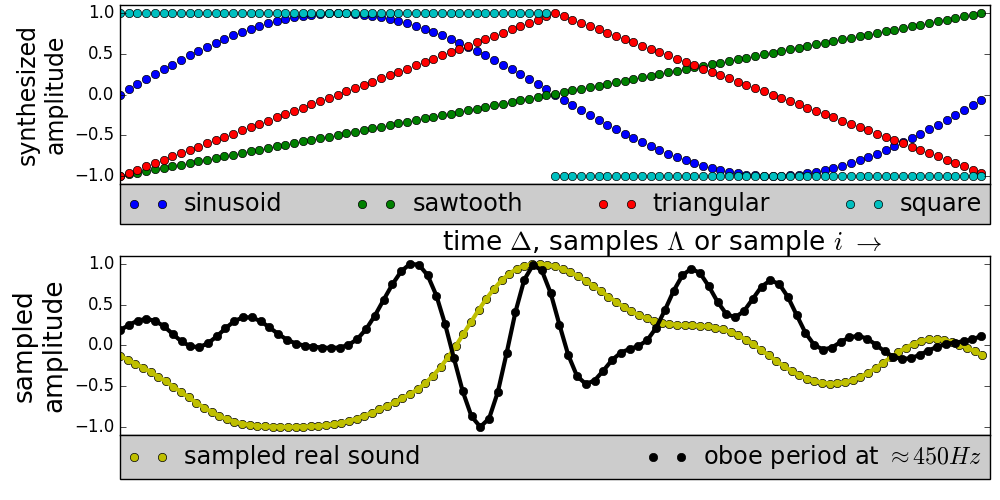
\includegraphics[width=.7\textwidth]{figures/waveForms__}
    \caption{Basic musical waveforms: (a) the basic synthetic  waveforms
	given by the Equations~\ref{sinusoid},~\ref{sawTooth},~\ref{triangular} and~\ref{square};
	(b) real waveforms.
	Because of the period with $\approx 100$ samples ($\lambda_f\approx 100$),
	if $f_s=44.1kHz$
	the basic and oboe waves have a fundamental frequency of $f=\frac{f_s}{\lambda_f}\approx \frac{44100}{100} = 441 \; Hz$,
	whatever the waveform is.}
        \label{fig:formasDeOnda}
\end{figure*}

The sequence $R=\{ r_i \}_0^{\lambda_f-1}$ of samples in a real sound (e.g. of Figure~\ref{fig:formasDeOnda}) can be taken as a basis for a sound $T^f$ in the following way:

\begin{equation}\label{sampleandoFormaDeOnda}
     T^f=\{ t_i^f \}=\Bigl\{ r_{(i\,\%\lambda_{f})} \Bigr\}
\end{equation}

The resulting sound has the spectrum of the original waveform.
As a consequence of the identical repetitions,
the spectrum is perfectly harmonic,
without noise or variations of the components
which are typical of natural phenomena.
This can be observed in Figure~\ref{fig:espectroOboe},
which shows the spectrum of the original oboe note and a note with the same duration,
whose samples consist of the repetition of the cycle on Figure~\ref{fig:formasDeOnda}.

\begin{figure*}
    \centering
        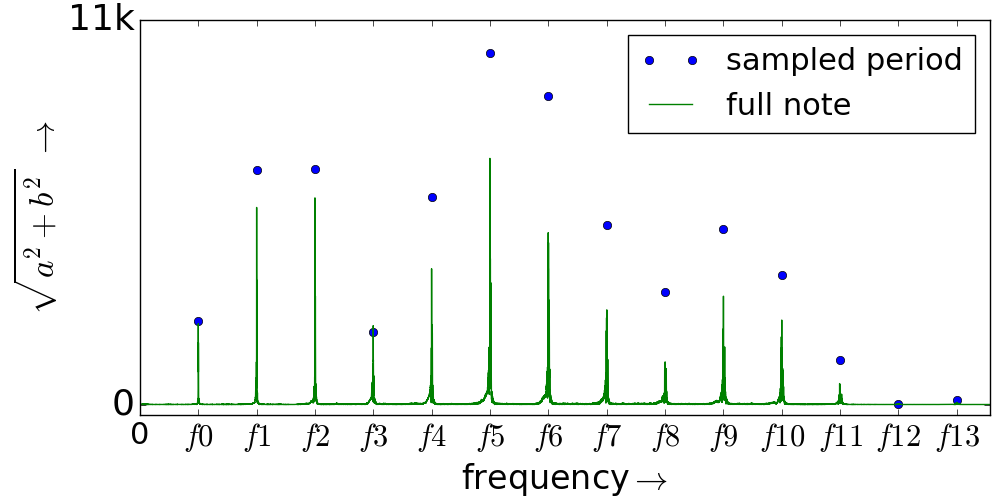
\includegraphics[width=.7\textwidth]{figures/oboeNaturalSampledSpectrum_}
	\caption{Spectra of the sonic waves of a natural oboe note and obtained through a sampled period. The natural sound has fluctuations in the harmonics and in its noise, while the sampled period note has a perfectly harmonic (and static) spectrum.}
        \label{fig:espectroOboe}
\end{figure*}

The simplest case is the spectrum with only one frequency, which is a sinusoid, often regarded as a ``pure'' oscillation (e.g. in terms of the \emph{simple harmonic motion}).
Let $S^f$ be a sequence whose samples $s_i^f$ describe a sinusoid with frequency $f$:

\begin{equation}\label{sinusoid}
     S^f=\{ s^f_i \}=\Bigl\{ \sin\bigl(2\pi \frac{i}{\lambda_f} \bigr)  \Bigr\} = \Bigl\{ \sin\bigl(2\pi f \frac{i}{f_s}\bigr)  \Bigr\} 
\end{equation}

\noindent where $\lambda_f=\frac{f_s}{f}=\frac{\delta_f}{\delta_s}$ is the number of samples in the period.

Other artificial waveforms are used in music for their spectral qualities and simplicity.
While the sinusoid is an isolated node in the spectrum, any other waveform presents a succession of harmonic components (harmonics).
Standard waveforms are specified by Equations~\ref{sinusoid},~\ref{sawTooth},~\ref{triangular} and~\ref{square}, and are illustrated in Figure~\ref{fig:formasDeOnda}.
These artificial waveforms are traditionally used in music for synthesis and oscillatory control of variables. They are also useful outside musical contexts~\cite{Openheim}.

The sawtooth presents all the harmonics with a decreasing energy of $-6dB/octave$\footnote{In 
musical jargon, an ``octave'' means a frequency and twice such frequency ($f$ and $2f$), or the bandwidth $[f,2f]$.}.
The sequence of temporal samples can be described as:

\begin{equation}\label{sawTooth}
	D^f=\left\{ d^f_i \right\}=\left\{ 2\frac{i\,\%(\lambda_f+1)}{\lambda_f} -1 \right\}
\end{equation}

The triangular waveform has only odd harmonics falling with $-12dB/octave$:
\begin{equation}\label{triangular}
     T^f=\left\{ t^f_i \right\}=\left\{1- \left| 2 - 4\frac{i\,\%\lambda_f}{\lambda_f} \right| \right\}
\end{equation}

The square wave also has only odd harmonics but falling at $-6dB/octave$:
\begin{equation}\label{square}
     Q^f=\left\{ q^f_i \right\}= \left\{
         \begin{array}{l l}
              1 & \quad \text{for } \; \; (i\,\%\lambda_f)   <  \lambda_f /2  \\
              -1 & \quad \text{otherwise}\\
         \end{array} \right.
\end{equation}

The square wave can be used in a subtractive synthesis with the purpose of mimicking a clarinet.
This instrument has only the odd harmonics and the square wave is convenient with its abundant energy at high frequencies.
The sawtooth is a common starting point for subtractive synthesis,
because it has both odd and even harmonics with high energy.
In general, these waveforms are appreciated as excessively rich in sharp harmonics,
and attenuation by filtering on treble and middle parts of the spectrum is 
especially useful for achieving a more natural and pleasant sound. 
The relatively attenuated harmonics of the triangle wave makes it the more functional 
- among the listed possibilities - to be used in the synthesis of musical notes without any further processing.
The sinusoid is often a nice choice, but a problematic one.
While pleasant if not loud in a very high pitch (above $\approx 500Hz$ it requires careful dosage),
the pitch of a pure sinusoid is not accurately detected by the human auditory system,
particularly at low frequencies.
Also, it requires a great amplitude gain for an increase in loudness of a sinusoid
if compared to other waveforms. Both particularities are understood in the scientific
literature as a consequence of the nonexistence of pure sinusoidal sounds in nature~\cite{Roederer}.
The spectra of each basic waveform is illustrated in Figure~\ref{fig:espectroDeOndas}.

\begin{figure*}
    \centering
        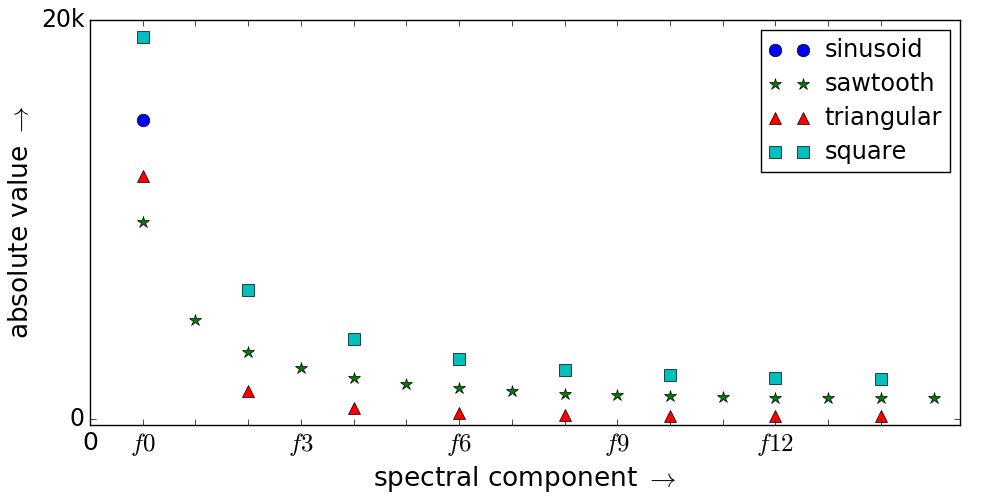
\includegraphics[width=.7\textwidth]{figures/waveSpectrum_}
    \caption{Spectra of basic artificial waveforms.
The isolated and exactly harmonic components of the spectra is a consequence of the fixed period.
	The figure exhibits the spectra described in Section~\ref{sec:timbre}:
	the sawtooth is the only waveform with a complete harmonic series (odd and even components);
	triangular and square waves have the same components (odd harmonics), decaying at $-12dB/octave$ and $-6dB/octave$, respectively;
	the sinusoid consists of a unique node in the spectrum.
	}
        \label{fig:espectroDeOndas}
\end{figure*}

This article has a Supporting Information document for describing the sinusoidal spectra of samples sounds and exemplifies by means of these basic waveforms~\cite{massNotesInMusic}.

\subsection{The basic note}\label{notaBasica}
In a nutshell,
a sequence $T$ of sonic samples separated by $\delta_a=1/f_s$ expresses a musical note with
a frequency of $f$ Hertz\footnote{Let $f$ be such that it divides $f_s$.
As mentioned before, this limitation simplifies the exposition for now
and will be overcome in the next section.} and $\Delta$ seconds of duration if,
and only if, it has the periodicity $\lambda_f=f_s/f$ and size $\Lambda=\lfloor f_s . \Delta \rfloor$:

\begin{equation}\label{eq:notaBasica}
T^{f,\; \Delta}=\{t_{i \, \% \lambda_f} \}_0^{\Lambda-1}= \left \{t^f_{i \; \% \left( \frac{f_s}{f} \right) } \right \}_0^{\Lambda-1}
\end{equation}

Such note still does not have a timbre: it is necessary to choose a waveform for the samples $t_i$ to have a value.
Any waveform can be used to further specify the note,
where $\lambda_f=\frac{f_s}{f}$ is the number of samples in each period.
Let $L^f \in \{S^f,Q^f,T^f,D^f,R^f \}$
(as given by Equations~\ref{sinusoid},~\ref{sawTooth},~\ref{triangular}
and~\ref{square} and let $R_i^f$ be a sampled waveform)
be the sequence that describes a period of the waveform 
 with duration $\delta_f=1/f$:

\begin{equation}\label{periodoUnico}
L^{f} = \left\{ l_i^f \right\}_0^{\delta_f . f_s -1}=\left\{ l_i^f \right\}_0^{\lambda_f-1}
\end{equation}

Thereafter, the sequence $T$ for a note of duration $\Delta$ and frequency $f$ is:

\begin{equation}\label{eq:notaBasicaTimbre}
T^{f,\; \Delta}=\left\{t_i^f\right\}_0^{\lfloor f_s . \Delta \rfloor -1}=\left \{ l^f_{i\,\%\left(\frac{f_s}{f}\right)} \right \}_0^{\Lambda-1}
\end{equation}

\subsection{Spatialization: localization and reverberation}\label{subsec:spac}
A musical note is always spatialized
(i.e. it is always produced within the ordinary three dimensional physical space)
even though it is not one of its four basic properties in canonical music theory (duration, loudness, pitch and timbre).
The consideration of this fact is the subject of the spatialization knowledge field and practice\footnote{By
spatialization one might find both:
1) the consideration of cues in sound that derive from the environment,
including the localization of the listener and the sound source;
2) techniques to produce sound through various sources, such as loudspeakers, singers and traditional musical instruments, for musical purposes.
We focus in the first issue although issues of the second are also tackled
and they are obviously intermingled.}.
A note has a source which has a three dimensional position.
This position is the spatial localization of the sound.
It is often (modeled as) a single point but can be a surface or a volume.
The reverberation in the environment in which a sound occurs is an important topic of spatialization.
Both concepts, spatial localization and reverberation,
are widely valued by composers, audiophiles and the music industry~\cite{floEsp}.

\subsubsection{Spatial localization}
It is understood that the perception of sound localization occurs in our nervous system
mainly by three cues: the delay of the incoming sound (and its reflections in the surfaces) between both ears,
the difference of sound intensity at each ear and the filtering performed by the human body,
specially in the chest, head and ears~\cite{Roederer, hrtf, Heeger}. 

\begin{figure}[h!]
    \centering
        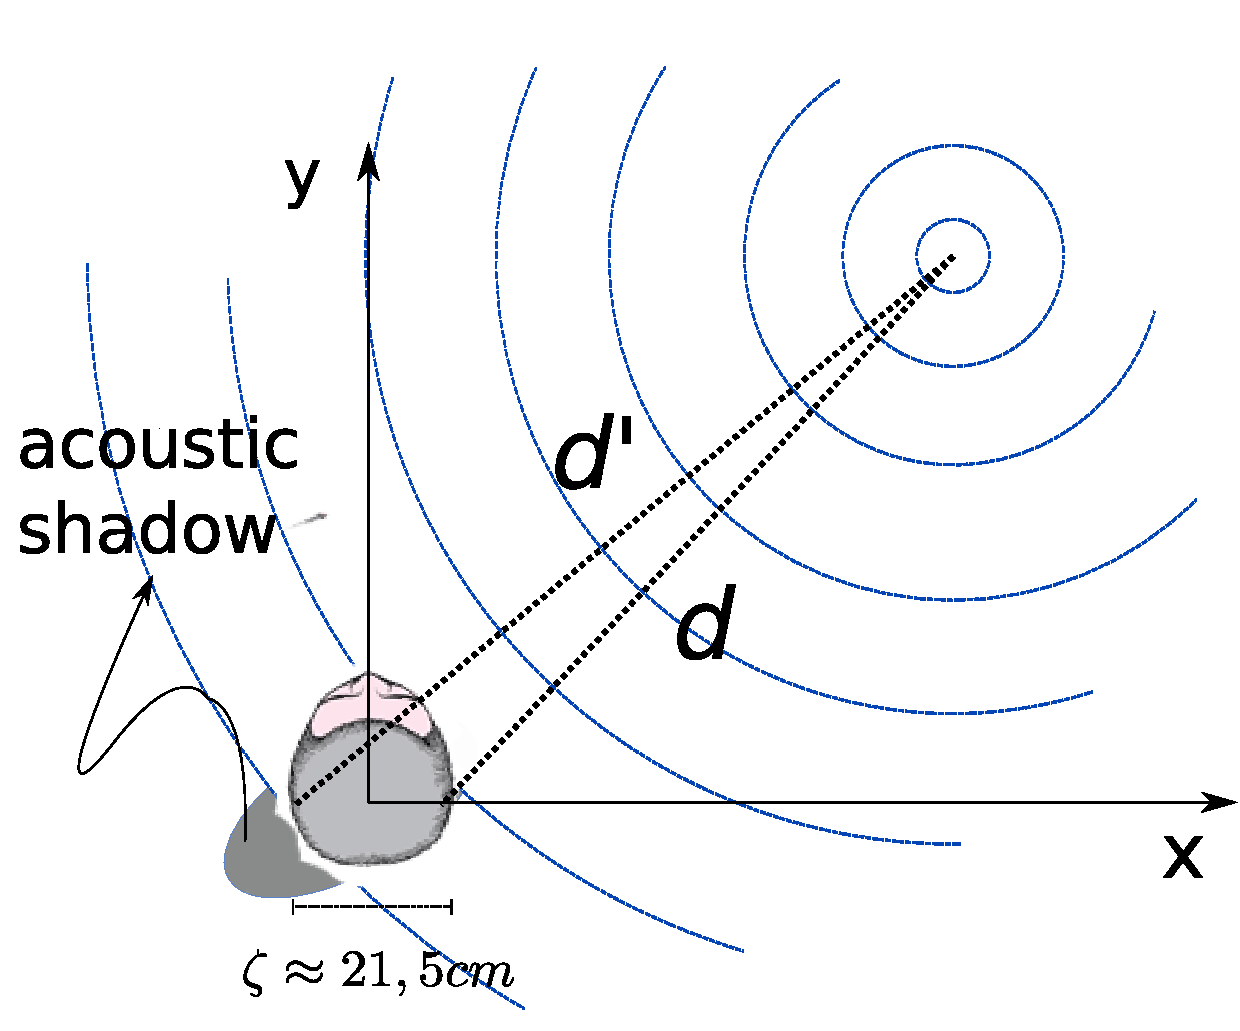
\includegraphics[width=.5\textwidth]{figures/espacializacao___}
    \caption{Detection of sound source localization: schema used to calculate the Interaural Time Difference (ITD) and the Interaural Intensity Difference (IID).}
    \label{fig:spac}
\end{figure}

An object placed at $(x,y)$, as in Figure~\ref{fig:spac}, is distant of each ear by:

\begin{equation}\label{eq:distOuvidos}
\begin{split}
d & =\sqrt{\left (x-\frac{\zeta}{2} \right )^2+y^2} \\
d' & =\sqrt{\left (x+\frac{\zeta}{2} \right )^2 + y^2}
\end{split}
\end{equation}

\noindent where $\zeta$ is the distance between the ears, known to be $\zeta \approx 21.5cm$ in an adult human.
The cues for the sonic localization are not easy to calculate, but,
in a very simplified model, useful for musical purposes,
straightforward calculations result in the Interaural Time Difference:

\begin{equation}\label{eq:dti}
ITD=\frac{d'-d}{v_{sound\;at\;air}\approx 343.2 }\quad \text{seconds}
\end{equation}

\noindent and in the Interaural Intensity Difference:

\begin{equation}\label{eq:dii}
IID=20\log_{10}\left (\frac{d}{d'}\right) \quad decibels
\end{equation}

$IID_a=\frac{d}{d'}$ can be used as a multiplicative constant to the right channel of a stereo sound signal
together with ITD~\cite{Heeger}:
\begin{equation}\label{eq:locImpl}
\begin{split}
\Lambda_{ITD} & = \left \lfloor \frac{d'-d}{343,2}  f_s \right \rfloor \\
IID_a & = \frac{d}{d'} \\
\left\{t_{(i+\Lambda_{ITD})}'\right\}_{\Lambda_{ITD}}^{\Lambda+\Lambda_{ITD}-1} & =\left\{IID_a . t_i\right\}_0^{\Lambda-1} \\
\left\{t_i'\right\}_0^{\Lambda_{ITD}-1} & = 0
\end{split}
\end{equation}

\noindent where,
where $\{t_i'\}$ are samples of the wave incident in the left ear, $\{t_i\}$ are samples for the right ear,
and $\Lambda_{ITD}=\lfloor ITD . f_s \rfloor$.
If $\Lambda_{ITD} < 0$, it is necessary to change $t_i$ by $t_i'$
and use $\Lambda_{ITD}'= | \Lambda_{ITD} |$ and $IID_a'=1 / IID_a$.

Spatial localization depends considerably on other cues.
By using only ITD and IID it is possible to specify solely
the horizontal angle (azimuthal) $\theta$ given by:

\begin{equation}\label{eq:angulo}
\theta=\arctan( y, x )
\end{equation}

\noindent with $x,y$ as presented in Figure~\ref{fig:spac}.
Notice that
the same pair of ITD and IID (as defined in Equations~\ref{eq:dti} and~\ref{eq:dii})
is related to all the points in a vertical circle parallel to
the head, i.e. the source can have any horizontal component inside the circle.
Such a circle is called the "cone of confusion".
In general, one can assume that the source is in the same horizontal plane
as the listener and at its front
(because humans are prone to hearing frontal and horizontal sources).
Even in such cases, there are other important cues for sound localization.
Consider the acoustic shadow depicted in Figure~\ref{fig:spac}:
for lateral sources the inference of the azimuthal angle is especially dependent
on the filtering of frequencies by the head, pinna (outer ear) and torso.
Also, low frequencies diffract and arrive to the opposite ear with a greater ITD. 
The complete localization, including height and distance of a sound source,
is given by the Head Related Transfer Function (HRTF).
There are well known open databases of HRTFs, such as CIPIC,
and it is possible to apply such transfer functions in a sonic 
signal by convolution (see Equation~\ref{eq:conv}).
Each human body has its own filtering and there are techniques 
to generate HRTFs to be universally used.~\cite{lazaSPA,CIPIC,floEsp,Heeger,hrtf} 

\subsubsection{Reverberation}
The reverberation results from sound reflections and absorption by the environment (e.g. a room) surface where a sound occurs.
The sound propagates through the air with a speed of $\approx 343.2m/s$ and can be emitted from a source with any directionality pattern. When a sound front encounters a surface there are: 1) inversion of the propagation speed component normal to the surface;  2) energy absorption, especially in high frequencies.
The sonic waves propagate until they reach inaudible levels (and further but then can often be neglected).
As a sonic front reaches the human ear, it can be described as the original sound, with the last reflection point as the source, and the absorption filters of each surface it has reached.
It is possible to simulate reverberations that are impossible in real systems.
For example, it is possible to use asymmetric reflections with relation to the axis perpendicular to the surface,
to model propagation in a space with more than three dimensions,
or consider a listener located in various positions.

There are reverberation models less related to each independent reflection and that explores valuable cues to the auditory system. In fact, reverberation can be modeled with a set of two temporal and two spectral regions~\cite{JOSPhy}:
\begin{itemize}
   \item First period: 'first reflections' are more intense and scattered.
   \item Second period: 'late reverberation' is practically a dense succession of indistinct delays with exponential decay and statistical occurrences.
   \item First band: the bass has some resonance bandwidths relatively spaced.
   \item Second band: mid and treble have a progressive decay and smooth statistical fluctuations.
\end{itemize}

Smith III states that usual concert rooms have a total reverberation time of $\approx 1.9$ seconds, and that the period of first reflections is around $0.1s$.
With these values, there are perceived wave fronts which propagate for $652.08m$ before reaching the ear.
In addition, sound reflections made after propagation for
$34.32m$ have incidences less distinct by hearing.
These first reflections are particularly important to spatial sensation.
The first incidence is the direct sound, described by ITD and IID e.g. as in Equations~\ref{eq:dti} and~\ref{eq:dii}.
Assuming that each one of the first reflections, before reaching the ear,
will propagate at least $3-30m$, depending on the room dimensions,
the separation between the first reflections is $8-90ms$.
Also, it is experimentally verifiable that the number of reflections increases with the square of time.
A discussion about the use of convolutions and filtering to favor the implementation of these phenomena is provided in Section~\ref{subsec:mus2}, particularly in the paragraphs about reverberation.~\cite{JOSPhy}

\subsection{Musical usages}\label{subsec:basMus}
Once the basic note is defined, it is didactically convenient to build musical structures with sequences based on these particles.
The sum of the amplitudes of $N$ sequences with same size $\Lambda$ results in the overlapped spectral contents of each sequence, in a process called mixing:

\begin{equation}\label{eq:mixagem}
\{t_i\}_0^{\Lambda-1}=\left \{ \sum_{k=0}^{N-1}t_{k,i} \right \}_0^{\Lambda-1}
\end{equation}

\begin{figure}[h!]
    {\centering
        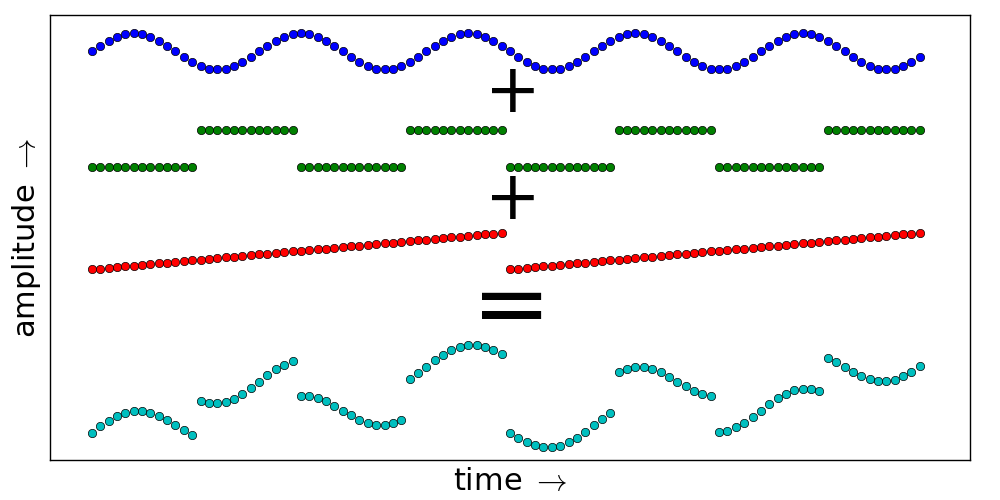
\includegraphics[width=.5\columnwidth]{figures/mixagem__}}
    \caption{Mixing of three sonic sequences. The amplitudes are directly summed sample-by-sample.}
        \label{fig:mixagem}
\end{figure}

Figure~\ref{fig:mixagem} illustrates this overlapping process of discretized sound waves, each with 100 samples. If $f_s=44.1kHz$, the frequencies of the sawtooth, square and sine wave are, respectively: $\frac{f_s}{100/2}=882Hz$, $\frac{f_s}{100/4}=1764Hz$ and $\frac{f_s}{100/5}=2205Hz$. The duration of each sequence is very short $\frac{f_s=44.1kHz}{100} \approx 2ms$. One can complete the sequence with zeroes to sum (mix) sequences with different sizes.

The mixed notes are generally separated by the ear according to the physical laws of resonance and by the nervous system~\cite{Roederer}.
This process of mixing musical notes results in musical harmony, where intervals between frequencies and chords of simultaneous notes guide subjective and abstract aspects of music appreciation~\cite{Harmonia} and are addressed in the Supporting Information document~\cite{massNotesInMusic}. 

Sequences can be concatenated in time. If the sequences $\{t_{k,i}\}_0^{\Lambda_k-1}$ represent musical notes,
their concatenation in a unique sequence $T$ is a simple melodic sequence (or melody):

\begin{equation}\label{eq:concatenacao}
\begin{split}
T = \{t_i\}_0^{\sum\Delta_k-1}= & \{t_{l,i}\}_0^{\sum\Delta_k-1}, \;\; \\ l\text{ smallest integer } : & \quad \Lambda_l > i -\sum_{j=0}^{l-1}\Lambda_j
\end{split}
\end{equation}

This mechanism is illustrated in Figure~\ref{fig:concatenacao} with the same sequences of Figure~\ref{fig:mixagem}. Although the sequences are short for the usual sample rates, it is easy to visually observe the concatenation of sonic sequences. In addition, each note has  a duration larger than $100ms$ if $f_s<1kHz$ (but need to oscillate faster to yield audible frequencies).

\begin{figure}[h!]
{    \centering
        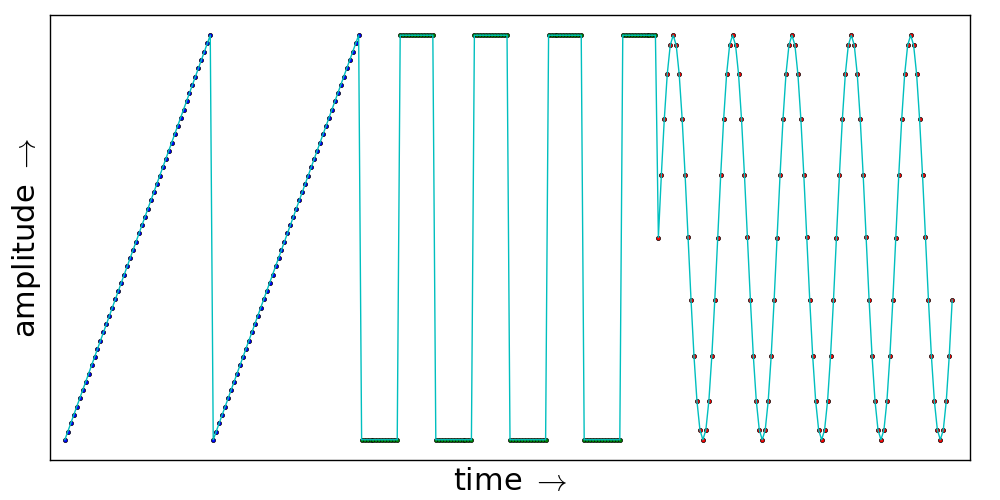
\includegraphics[width=.5\columnwidth]{figures/concatenacao__}}
    \caption{Concatenation of three sounds.}
        \label{fig:concatenacao}
\end{figure}

The musical piece \emph{reduced-fi} explores the temporal juxtaposition of notes, resulting in a homophonic piece.
The vertical principle (mixing) is demonstrated at the \emph{sonic portraits}, static sounds with peculiar spectrum.~\cite{MASSA}

With the basic musical note in discrete-time audio carefully described, the next section develops the temporal evolution of its contents as in \emph{glissandi} and intensity envelopes. Filtering of spectral components and noise generation complements the musical note as a self-contained unit. The Supporting Information Document~\cite{massNotesInMusic} is dedicated to the organization of these notes e.g. by using metrics and trajectories, with regards to traditional music theory.


\section{Variation in the basic note}\label{sec:internalVar}\label{sec:varInternas}
The basic digital music note defined in Section~\ref{sec:notaDisc} has the following parameters: duration, pitch, intensity (loudness) and timbre. This is a useful and paradigmatic model, but it does not exhaust all the aspects of a musical note. First of all, characteristics of the note change along the note itself~\cite{Chowning}. For example, a $3s$ piano note has intensity with an abrupt rise at the beginning and a progressive decay, has spectral variations with harmonics decaying and some others emerging along time. These variations are not mandatory, but they are used in sound synthesis for music because they reflect how sounds appear in nature. This is considered so important that there is a rule of thumb: to make a sound that incites interest by itself, arrange internal variations on it~\cite{Roederer}.
To explore all the ways by which variations occur within a note is out of the scope of any work, given the sensibility of the human ear and the complexity of human sound cognition. In this section, primary resources are presented to produce variations in the basic note. It is worthwhile to recall that all the relations in this and other sections are implemented in Python and published in public domain. All relations described in this section are implemented in the file \texttt{src/sections/3.py}.
The musical pieces related to this section are on the directory~\texttt{src/pieces3/}.~\cite{MASSA}
 
\subsection{Lookup table}\label{subsec:lookup}
The \emph{Lookup Table} (LUT) is an array for indexed operations which substitutes continuous and repetitive calculations.
It is used to reduce computational complexity and for employing functions without calculating them directly, e.g. from sampled data or hand picked values.
In music its usage simplifies many operations and enables the use a single wave period to synthesize sounds in the whole audible spectrum, with any waveform.

Let $\widetilde{\Lambda}$ be the wave period in samples and $\widetilde{L} = \left\{\, \widetilde{l}_i \,\right\}_0^{\widetilde{\Lambda} -1}$ the sample sequence with the waveform.
A sequence $T^{f,\,\Delta}$ with samples of a sound with frequency $f$ and duration $\Delta$ can be obtained by means of $\widetilde{L}$:

\begin{figure*}[t!]
    \centering
        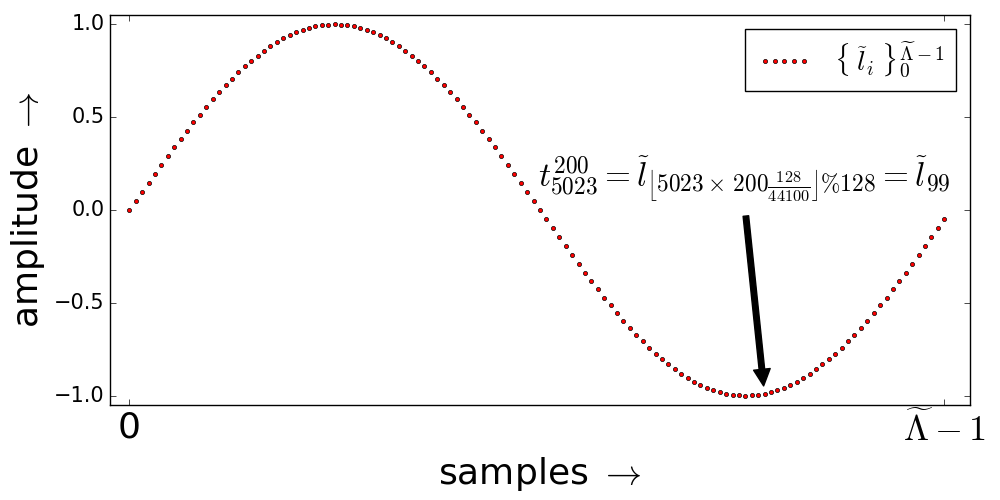
\includegraphics[width=.7\textwidth]{figures/lut_}
	\caption{Search (lookup) in a reference table (\emph{lookup table} or LUT) to synthesize sounds at different frequencies using a unique waveform with high resolution.
	Each \emph{i-th} sample $t_i^f$ of a sound with frequency $f$ is related to the samples in the table $\widetilde{L}=\{\widetilde{l}_i\}_0^{\widetilde{\Lambda}-1}$ by $t_i^{f}=\widetilde{l}_{\left\lfloor i f\frac{\widetilde{\Lambda}}{f_s} \right\rfloor \%\,\widetilde{\Lambda}}$ where $f_s$ is the sampling rate.}
        \label{fig:lut}
\end{figure*}

\begin{equation}\label{eq:lut}
\begin{split}
T^{f,\,\Delta}=\left\{t_i^f\right\}_0^{\lfloor \, f_s . \Delta \, \rfloor -1} = \left\{ \, \widetilde{l}_{\gamma_i \% \widetilde{\Lambda} }\, \right\}_{0}^{\Lambda-1}\; , \quad \text{where} \;\; \gamma_i = \left \lfloor i f \frac{ \widetilde{\Lambda}}{f_s} \right \rfloor  
\end{split}
\end{equation}

In other words, with the right LUT indexes ($\gamma_i\%\widetilde{\Lambda}$) it is possible to synthesize sounds at any frequency.
Figure~\ref{fig:lut} illustrates the calculation of a sample $t_i$ from $\left\{\,\widetilde{l}_i\,\right\}$ for $f=200Hz$, $\widetilde{\Lambda}=128$ and adopting the sample rate of $f_s=44.1kHz$. Though this is not a practical configuration (as discussed below), it allows for a graphical visualization of the procedure.

The calculation of the integer $\gamma_i$ introduces noise which decreases as $\widetilde{\Lambda}$ increases.
In order to use this calculation in sound synthesis,
with $f_s=44.1 kHz$, the standard guidelines suggest the use of $\widetilde{\Lambda} = 1024$ samples,
yielding a noise level of $\approx -60dB$.
Larger tables might be used to achieve sounds with a greater quality.
Also, a rounding or interpolation method can be used,
but we advocate the use of a larger table since it does not
introduce relevant computation overhead.~\cite{Geiger}

The expression defining the variable $\gamma_i$ can be understood as $f_s$ being added to $i$ at each second.
If $i$ is divided by the sample frequency, $\frac{i}{f_s}$
is incremented by $1$ at each second. Multiplied by the period, it results in $i \frac{\widetilde{\Lambda}}{f_s}$, which covers the period in one second.
Finally, with frequency $f$ it results in $i f \frac{\widetilde{\Lambda}}{f_s}$ which completes $f$ periods $\widetilde{\Lambda}$ in $1$ second, i.e. the resulting sequence presents the fundamental frequency $f$.

There are important considerations here: it is possible to use practically any frequency $f$.
Limits exist only at low frequencies when the size of table $\widetilde{\Lambda}$ is not sufficient for the sample rate $f_s$.
The lookup procedure is virtually costless and replaces calculations by simple indexed searches 
(what is generally understood as an optimization process).
Unless otherwise stated, this procedure will be used along all the following discussions for every applicable case.
LUTs are broadly used in computational implementations for music,
and are known also as wavetables.
A classical usage of LUTs is known as \emph{Wavetable Synthesis},
which generally consists of many LUTs used together to generate a quasi-periodic musical note~\cite{Cook,Wavetable}.

\subsection{Incremental variations of frequency and intensity}\label{subsec:vars}
As stated by the (Weber and) Fechner law~\cite{Weber-Fechner},
human perception holds a logarithmic relation to stimulus.
That is to say, the exponential progression of a stimulus is perceived as linear.
For didactic reasons, and given its use in AM and FM synthesis (Section~\ref{subsec:tvaf}), linear variation is discussed first.

Consider a note with duration $\Delta = \frac{\Lambda}{f_s}$, in which the frequency $f=f_i$ varies linearly from $f_0$ to $f_{\Lambda -1}$. Thus:

\begin{equation}\label{freqLinear}
 F=\{f_i\}_0^{\Lambda-1}=\left\{f_0 + (f_{\Lambda-1}-f_0)\frac{i}{\Lambda-1} \right\}_0^{\Lambda-1}
\end{equation}

\begin{equation}\label{indiceLinear}
\begin{split}
	\Delta_{\gamma_i}=\frac{\widetilde{\Lambda}}{f_s}f_i \quad \Rightarrow \quad \gamma_i & = \left \lfloor \sum_{j=0}^{i} \frac{\widetilde{\Lambda}}{f_s}f_j \right \rfloor \\
	\gamma_i & =  \left \lfloor \sum_{j=0}^{i} \frac{\widetilde{\Lambda}}{f_s} \left [f_0 + (f_{\Lambda-1}-f_0)\frac{j}{\Lambda-1} \right ] \right \rfloor 
\end{split}
\end{equation}

\begin{equation}\label{serieAmostralLin}
 \left\{t_i^{\;\overline{f_0,\, f_{\Lambda-1}}}\right\}_0^{\Lambda-1}=\left\{\,\widetilde{l}_{\gamma_i \% \widetilde{\Lambda}}\,\right\}_0^{\Lambda-1}
\end{equation}

\noindent where $\Delta_{\gamma_i}=f_i\frac{\widetilde{\Lambda}}{f_s}$ is the LUT increment between two samples given the sound frequency of the first sample.
There is a general rule to be noticed here: when a sound has variations in the fundamental frequency,
one should account for them in the LUT indexing.
The resulting indexes can be found by a cumulative sum of each indexing displacement.
The equations for linear pitch transition are:

\begin{equation}\label{freqExponencial}
 F=\{f_i\}_0^{\Lambda-1}=  \left\{f_0 \left ( \frac{f_{\Lambda-1}}{f_0} \right ) ^{\frac{i}{\Lambda -1}} \right\}_0^{\Lambda-1}
\end{equation}

\begin{equation}\label{indiceExponencial}
\begin{split}
 \Delta_{\gamma_i}= \frac{\widetilde{\Lambda}}{f_s}f_i \quad \Rightarrow  \quad \gamma_i= & \left \lfloor \sum_{j=0}^{i} \frac{\widetilde{\Lambda}}{f_s}f_j \right \rfloor \\
	\gamma_i = & \left \lfloor \sum_{j=0}^{i} f_0 \frac{\widetilde{\Lambda}}{f_s} \left ( \frac{f_{\Lambda-1}}{f_0} \right ) ^{\frac{j}{\Lambda -1}} \right \rfloor
\end{split}
\end{equation}

\begin{equation}\label{serieAmostralLog}
 \left\{t_i^{\;\overline{f_0,\,f_{\Lambda-1}}}\right\}_0^{\Lambda-1}=\left\{\,\widetilde{l}_{\gamma_i \% \widetilde{\Lambda}}\,\right\}_0^{\Lambda-1}
\end{equation}

\begin{figure}[h!]
     \centering
         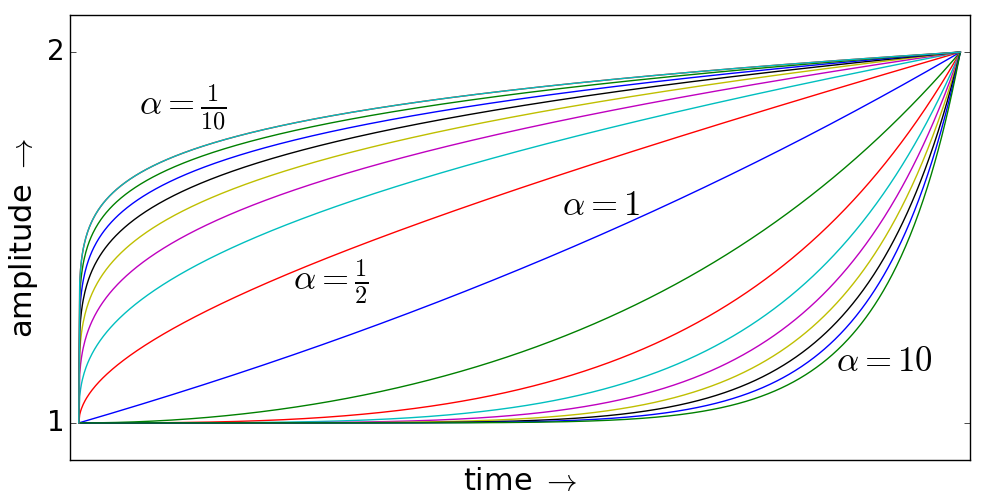
\includegraphics[width=.7\columnwidth]{figures/transicao_}
     \caption{Intensity transitions for different values of $\alpha$ (see Equations~\ref{seqAmp} and~\ref{transAmp}).}
         \label{fig:transicao}
\end{figure}

The term $\frac{i}{\Lambda-1}$ covers the interval $[0,1]$ and it is possible to raise it to a power $\alpha\geq0$ in such a way that the beginning of the transition will be smoother or steeper.
This procedure is especially useful for energy variations with the purpose of changing the loudness\footnote{See Section~\ref{subsec:volume} for considerations about loudness, amplitudes and decibels.}.
Thus, for amplitude variations:
\begin{equation}\label{seqAmp}
\begin{split}
 \{a_i\}_0^{\Lambda-1}= \left \{ a_0 \left ( \frac{a_{\Lambda-1}}{a_0} \right )^{\left ( \frac{i}{\Lambda-1} \right )^\alpha} \right \}_0^{\Lambda-1}= \left \{ \left ( {a_{\Lambda-1}} \right )^{\left ( \frac{i}{\Lambda-1} \right )^\alpha} \right \}_0^{\Lambda-1}
\end{split}
\end{equation}
where $a_0$ is the initial amplitude factor and
$a_{\Lambda-1}$ is an amplitude factor to be reached at the end of the transition.
Applying the loudness transition to a sonic sequence $T$:

\begin{equation}\label{transAmp}
\begin{split}
 T^{'}=T \odot A = \{t_i . a_i\}_0^{\Lambda-1} = \left \{ t_i . (a_{\Lambda-1} )^{\left ( \frac{i}{\Lambda-1} \right )^\alpha} \right \}_0^{\Lambda-1}
\end{split}
\end{equation}

It is often convenient to have $a_0=1$ to start a new sequence with the original amplitude and then progressively change it.
If $\alpha=1$, the amplitude variation follows the exponential progression that is related to the linear variation of loudness. Figure~\ref{fig:transicao} depicts transitions between values 1 and 2 and for different values of $\alpha$, a gain of $\approx 6dB$ as given by Equation~\ref{eq:ampVol}.

Special attention should be given while considering $a=0$.
In Equation~\ref{seqAmp}, $a_0=0$ results in a division by zero and if $a_{\Lambda-1}=0$, there will be a multiplication by zero.
Both cases make the procedure useless, once a ratio of any number in relation to zero is not well defined for our purposes. It is possible to solve this dilemma choosing a number that is small enough like $-80dB\;\Rightarrow a=10^{\frac{-80}{20}}=10^{-4}$ as the minimum loudness for a \emph{fade in} ($a_0=10^{-4}$) or for a \emph{fade out} ($a_{\Lambda-1}=10^{-4}$). A linear fade can be used then to reach zero amplitude, if needed. Another common solution is the use of the quartic polynomial term $x^4$, as it reaches zero without these difficulties and gets reasonably close to the curve with $\alpha=1$ as it departs from zero~\cite{Cook}.

Using Equations~\ref{ampDec} and~\ref{transAmp} to specify a transition of $V_{dB}$ decibels:

\begin{equation}\label{seqAmpDB}
T^{'}=\left\{ t_i 10^{\frac{V_{dB}}{20}\left( \frac{i}{\Lambda-1} \right)^\alpha} \right\}_0^{\Lambda-1}
\end{equation}

\noindent in the general case of amplitude variations following a geometric progression. The greater the value of $\alpha$, the smoother the sound introduction and more intense its end. $\alpha>1$ results in loudness transitions commonly called \emph{slow fade}, while $\alpha<1$ results in \emph{fast fade}~\cite{guillaume}.

For linear amplification -- but not linear perception -- it is sufficient to use an appropriate sequence $\{a_i\}$:

\begin{equation}\label{seqAmpLin}
a_i=a_0 + (a_{\Lambda-1}-a_0)\frac{i}{\Lambda-1}
\end{equation}

The linear transitions will be used for AM and FM synthesis, while exponential transitions are proper for tremolos and vibratos, as developed in Section~\ref{subsec:tvaf}. A non-oscillatory exploration of these variations is in the music piece \emph{ParaMeter Transitions}~\cite{MASSA}.

\subsection{Application of digital filters}\label{subsec:filtros}
This subsection is limited to a description of sequences processing by convolution and difference equations, and immediate applications, as a thorough discussion of filtering is beyond the scope of this study\footnote{The implementation of filters encompasses an area of recognized complexity, with dedicated literature and software~\cite{Openheim,smith}.}.
With this procedure it is possible to achieve reverberators, equalizers, \emph{delays}, to name a few of a variety of other filters for sound processing used to obtain musical/artistic effects.
Filter employment can be part of the synthesis process or made subsequently as part of processes commonly referred to as ``acoustic/sound treatment''.


\subsubsection{Convolution and finite impulse response (FIR) filters}\label{subsec:conv}
\begin{figure*}
     \centering
         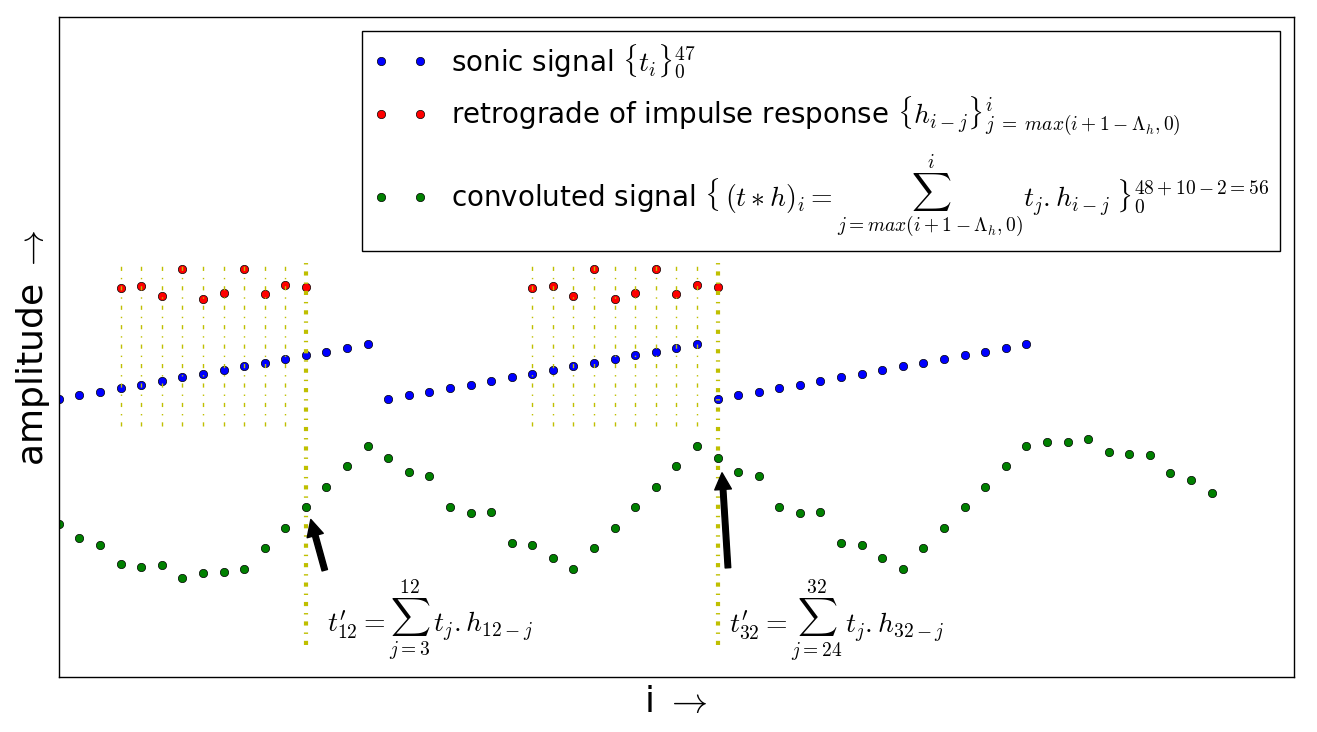
\includegraphics[width=\textwidth]{figures/convolucao_}
     \caption{Graphical interpretation of convolution. Each resulting sample is the sum of the previous samples of a signal, with each one multiplied by the retrograde of the other sequence.}
         \label{fig:conv}
\end{figure*}

Filters applied by means of convolution are known by the acronym FIR (Finite Impulse Response) and are characterized by having a finite sample representation.
This sample representation is called `impulse response' $\{h_i\}$.
FIR filters are applied in the time domain by means of convolution of the sound with the respective impulse response of the filter.
For the purposes of this work, convolution of $T$ with $H$ is defined as:

\begin{equation}\label{eq:conv}
 \begin{split}
 \left\{t_i'\right\}_0^{\Lambda_t+\Lambda_h-2\; = \;\Lambda_{t\, '}-1} = & \{(T*H)_i\}_0^{\Lambda_{t \, '}-1} = \{(H*T)_i\}_0^{\Lambda_{t \, '}-1} \\
     = & \left \{ \sum_{j=0}^{min(\Lambda_h-1,i)}h_{j} t_{i-j} \right \}_0^{\Lambda_{t\, '}-1} 
     \\ = & \left \{ \sum_{j=max(i+1-\Lambda_h,0)}^{i}t_j h_{i-j} \right \}_0^{\Lambda_{t\, '}-1}
 \end{split}
\end{equation}

\noindent where $t_i=0$ for the samples not given.
In other words, the sound $\{t_i'\}$, resulting from the convolution of $\{t_i\}$, with the impulse response $\{h_i\}$, has each $i$-th sample $t_i$ overwritten by the sum of its last $\Lambda_h$ samples $\{t_{i-j}\}_{j=0}^{\Lambda_h-1}$ multiplied one-by-one by samples of the impulse response $\{h_i\}_0^{\Lambda_h-1}$. This procedure is illustrated in Figure~\ref{fig:conv}, where the impulse response $\{h_i\}$ is in its retrograde form, and $t_{12}'$ and $t_{32}'$ are two samples calculated using the convolution given by $(T*H)_i=t_i'$. The final signal always has the length of $\Lambda_t+\Lambda_h -1=\Lambda_{t'}$.
It is also possible to apply the filter by multiplying the Fourier coefficients of both the sound and the impulse response,
and then performing the inverse Fourier transform~\cite{Openheim}.
This application of the filter in the frequency domain is usually much faster
especially when using a Fast Fourier Transform (FFT) routine.

The impulse response can be provided by physical measurement or by pure synthesis.
An impulse response for a reverberation, for example, can be obtained by recording the sound of the environment when someone triggers a click which resembles an impulse, or obtained by a sinusoidal sweep whose Fourier transform approximates its frequency response.
Both are impulse responses which, properly convoluted with the sonic sequence, result in the same sound with a reverberation that resembles the original environment where the measurement was made~\cite{Cook}.

The Fourier transform of an impulse response of a FIR filter is
an even and real envelope.
Convoluted with a sound (in the time or frequency domain), it performs the frequency filtering specified by the envelope.
The greater the number of samples, the higher the envelope resolution and the computational complexity, which should often be weighted, for convolution is expensive.

An important property is the time shift caused by convolution with a shifted impulse. Despite being computationally expensive, it is possible to create \emph{delay lines} by means of a convolution with an impulse response that has an impulse for each intended re-incidence of the sound. Figure~\ref{fig:delays} shows the shift caused by convolution with an impulse. Depending on the density of the impulses, the result is perceived as rhythm (from an impulse for each couple of seconds to about 20 impulses per second) or as pitch (from about 20 impulses per second and higher densities). In the latter case, the process is considered e.g. granular synthesis, reverberation or equalization.

\begin{figure*}
    \centering
        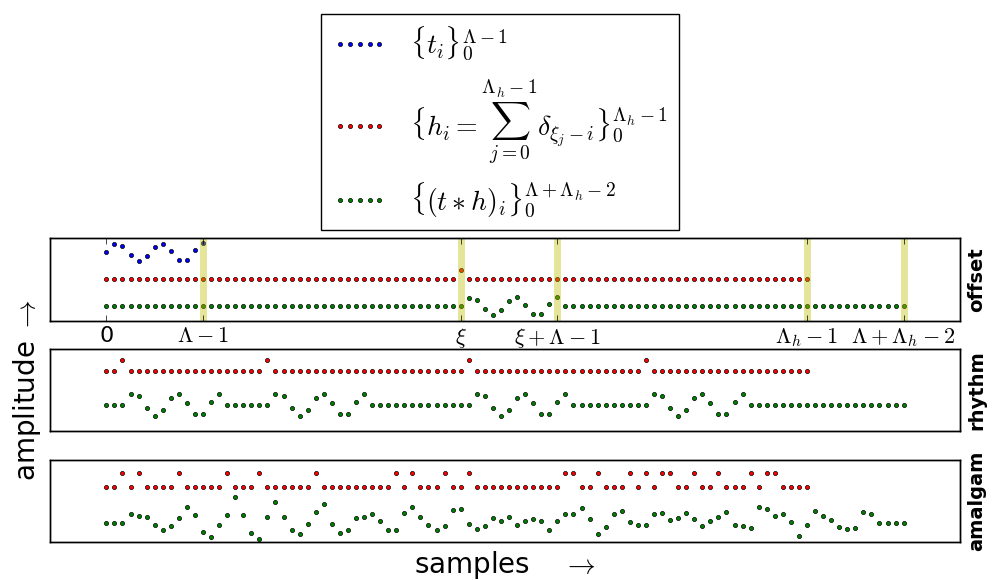
\includegraphics[width=\textwidth]{figures/delays_}
    \caption{Convolution with different densities of impulses: shifting (a), delay lines (b) and granular synthesis~(c).
    The vertical axis is related to amplitude although one should keep in mind that each subplot has two or three displaced signals.}
        \label{fig:delays}
\end{figure*}

\subsubsection{Infinite impulse response (IIR) filters}
This class of filters, known by the acronym IIR, is characterized by having an infinite time representation, i.e.\ the impulse response does not converge to zero. Its application is usually made by the following equation:

\begin{equation}\label{eq:diferencas}
 t_i' = \frac{1}{b_0}\left ( \sum_{j=0}^Ja_j t_{i-j} + \sum_{k=1}^Kb_k t_{i-k}' \right )
\end{equation}

The variables may be normalized: $a_j'=\frac{a_j}{b_0}$ and $b_k'=\frac{b_k}{b_0} \Rightarrow b_0' = 1$.
Equation~\ref{eq:diferencas} is called `difference equation' because the resulting samples 
$\left\{t_i'\right\}$ are given by weighted differences between original samples $\{t_i\}$ 
and previous ones in the resulting signal $\left\{t_{i-k}'\right\}$.

There are many methods and tools to obtain IIR filters. The text below lists a selection for didactic purposes and as a reference. They are well behaved filters and their main characteristics are described in Figure~\ref{fig:iir}. For filters of simple order, the cutoff frequency $f_c$ is where the filter performs an attenuation of $-3dB \approx 0.707 $ of the original amplitude.
For band-pass and band-reject (or 'notch') filters, this attenuation has two specifications: $f_c$ (in this case, the `center frequency') and bandwidth $bw$. In both frequencies $f_c \pm bw$ there is an attenuation of $-3dB \approx 0.707$ of the original amplitude.
There is sound amplification in band-pass and band-reject filters when the cutoff frequency is low and the bandwidth is large enough. In trebles, these filters present only a deviation of the expected profile, extending the envelope to the bass.

It is possible to apply filters successively in order to obtain filters with other frequency responses. Another possibility is to use a biquad 'filter recipe'\footnote{Short for 'biquadratic': its transfer function has two poles and two zeros, i.e. its first direct form consists of two quadratic polynomials in the fraction: $\mathbb{H}(z)=\frac{a_0+a_1.z^{-1}+a_2.x^{-2}}{1- b_1.z^{-1} -b_2 . z^{-2}}$.} or the calculation of Chebichev filter coefficients\footnote{Butterworth and Elliptical filters can be considered as special cases of Chebichev filters~\cite{Openheim,smith}.}.
Both alternatives are explored by~\cite{JOSFM,smith}, and by the collection of filters maintained by the \emph{Music-DSP} community of the Columbia University~\cite{music-dsp,Openheim}.

\begin{figure*}
    \centering
        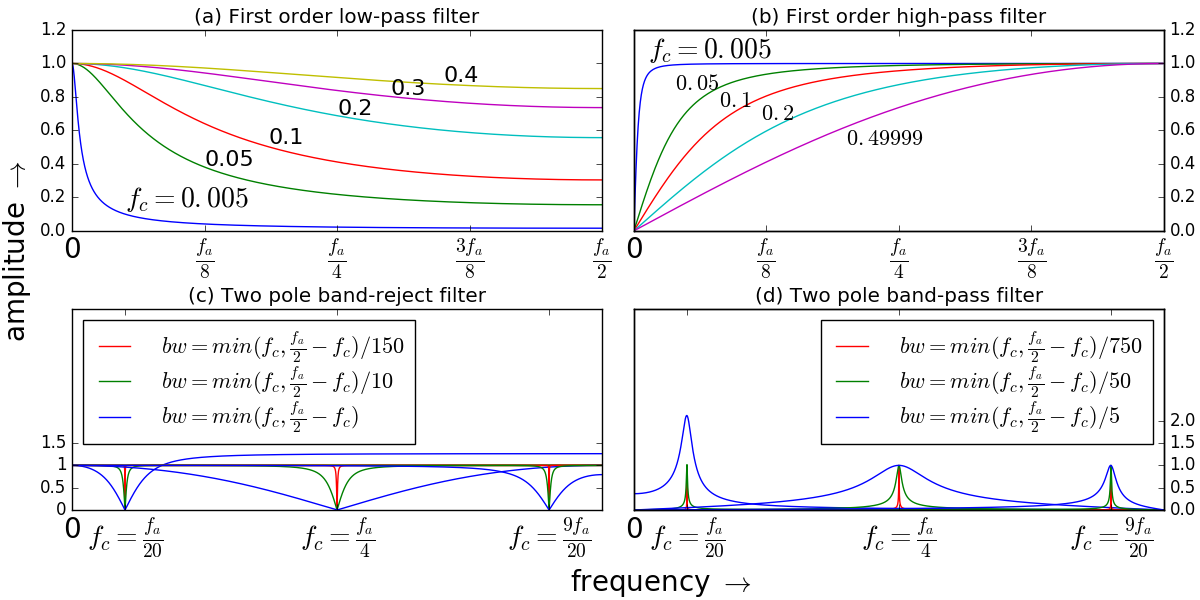
\includegraphics[width=\textwidth]{figures/iir__}
    \caption{Moduli for the frequency response (a), (b), (c) and (d) for IIR filters of Equations~\ref{eq:passa-baixas},~\ref{eq:passa-altas},~\ref{eq:passa-banda} and~\ref{eq:rejeita-banda} respectively, considering different cutoff frequencies, center frequencies and bandwidth.}
        \label{fig:iir}
\end{figure*}

\begin{enumerate}
  \item Low-pass with a simple pole, module of the frequency response in the upper left corner of Figure~\ref{fig:iir}. The general equation has the cutoff frequency $f_c \in (0,\frac{1}{2})$, fraction of the sample frequency $f_s$ in which an attenuation of $3dB$ occurs. The coefficients $a_0$ and $b_1$ of the IIR filter are given by $x \in [e^{-\pi},1]$:
\begin{equation}\label{eq:passa-baixas}
 \begin{split}
 x & =e^{-2\pi f_c} \\
 a_0 & =  1-x \\
 b_1 & =  x
 \end{split}
\end{equation}
  \item High-pass filter with a simple pole, module of its frequency responses at the upper right corner of Figure~\ref{fig:iir}. The general equation with cutoff frequency $f_c \in (0,\frac{1}{2})$ is calculated by means of $x \in [e^{-\pi},1]$:
\begin{equation}\label{eq:passa-altas}
 \begin{split}
 x & =e^{-2\pi f_c} \\
 a_0 & =  \frac{x+1}{2} \\
 a_1 & =  -\frac{x+1}{2} \\
 b_1 & =  x
 \end{split}
\end{equation}
\item Notch filter.
This filter is parametrized by a center frequency $f_c$ and bandwidth $bw$, both given as fractions of $f_s$, therefore $f,\; bw \in (0,\frac{1}{2})$.
Both frequencies $f_c \pm bw$ have $\approx 0.707$ of the amplitude, i.e.
an attenuation of $3dB$.
The auxiliary variables $K$ and $R$ are:
\begin{equation}\label{eq:varAux}
 \begin{split}
  R & = 1 - 3bw \\
  K & = \frac{1-2R\cos(2\pi f_c) + R^2}{2 - 2 \cos (2 \pi f_c)}
 \end{split}
\end{equation}
The band-pass filter in the lower left corner of Figure~\ref{fig:iir} has the following coefficients:
\begin{equation}\label{eq:passa-banda}
 \begin{split}
 a_0 & =  1 - K \\
 a_1 & =  2(K-R)\cos (2\pi f_c) \\
 a_2 & =  R^2-K \\
 b_1 & =  2R \cos (2\pi f_c) \\
 b_2 & =  -R^2
 \end{split}
\end{equation}
The coefficients of band-reject filter, depicted in the lower right of Figure~\ref{fig:iir}, are:
\begin{equation}\label{eq:rejeita-banda}
 \begin{split}
 a_0 & =  K \\
 a_1 & =  -2K\cos (2\pi f_c) \\
 a_2 & =  K \\
 b_1 & =  2R \cos (2\pi f_c) \\
 b_2 & =  -R^2
\end{split}
\end{equation}
\end{enumerate}

\subsection{Noise}\label{subsec:ruidos}
Sounds without an easily recognizable pitch are generally called noise~\cite{Lacerda}. They are important musical sounds, as noise is present in real notes, e.g. emitted by a violin or a piano. Furthermore, many percussion instruments do not exhibit an unequivocal pitch and their sounds are generally regarded as noise~\cite{Roederer}. In electronic music, including electro-acoustic and dance genres, noise has diverse uses and frequently characterizes the music style~\cite{Cook}. 

The absence of a definite pitch is due to the lack of a perceptible harmonic organization in the sinusoidal components of the sound.
Hence, there are many ways to generate noise. The use of random values to generate the sound sequence $T$ is a trivial method but not outstandingly useful because it tends to produce white noise with little or no variations~\cite{Cook}. Another possibility to generate noise is by using the desired spectrum, from which it is possible to perform the inverse Fourier transform. The spectral distribution should be done with care: if phases of components present prominent correlation, the synthesized sound will concentrate energy in some portions of its duration.

\begin{figure*}
	\hspace*{-.75cm}
         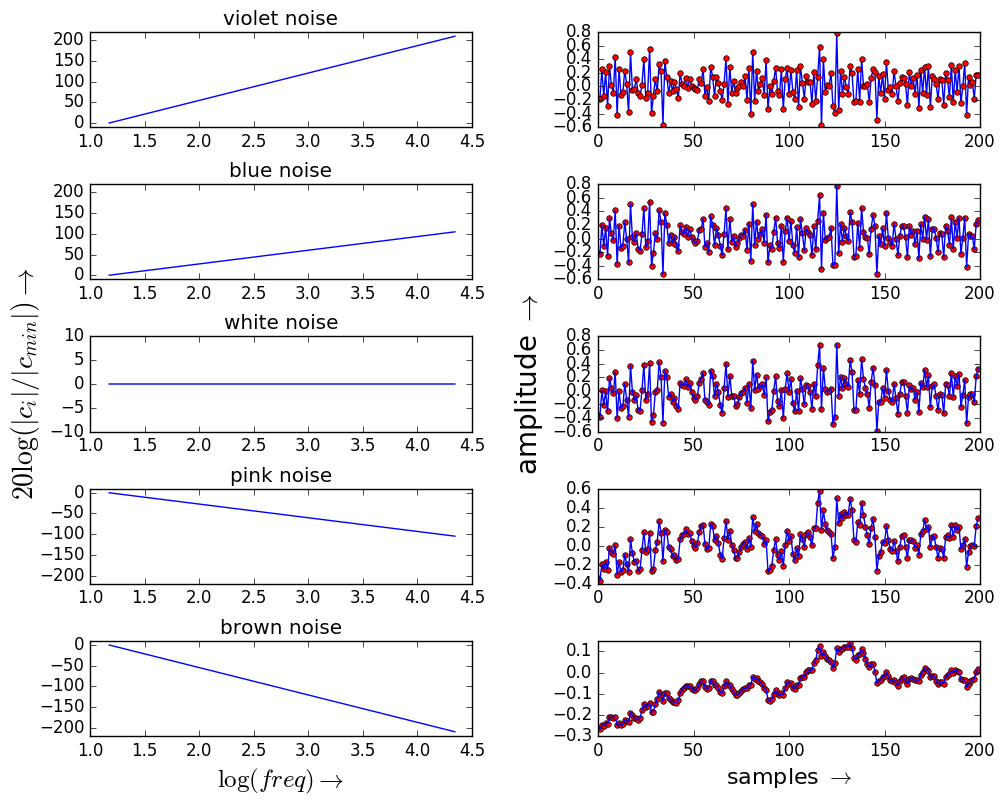
\includegraphics[width=1.\textwidth]{figures/ruidos_}
     \caption{Colors of noise generated by Equations~\ref{eq:branco},~\ref{eq:rosa},~\ref{eq:marrom},~\ref{eq:azul} and~\ref{eq:violeta}: spectrum and example waveforms.}
         \label{fig:ruidos}
\end{figure*}

Some noises with static spectra are listed below. They are called \emph{colored noise} since they are associated with colors for many reasons.
Figure~\ref{fig:ruidos} shows the spectral profile and the corresponding sonic sequence side-by-side. All five noises were generated with the same phase for each component, making it straightforward to observe the contributions of different parts of the spectrum.

\begin{itemize}
 \item The white noise has this name because its energy is distributed equally among all frequencies, such as the white color. It is possible to obtain white noise with the inverse transform of the following coefficients:
\begin{equation}\label{eq:branco}
 \begin{split}
f_{\text{min}} & \approx 15 Hz \\
f_i  &= i \frac{f_s}{\Lambda} \;, \;\; \quad i \;\leq\; \frac{\Lambda}{2},\;\; i\;\in\;\mathbb{N}  \\
c_i & =0\;,\;\; \forall \; i \; : f_i<f_{\text{min}} \\
% c_i & =e^{j.x}\;,\; x \; \text{random} \; \in \; [0,2\pi]\;,\; i \; \in \; \left[1, \, \frac{\Lambda}{2}-1\right] \\
c_i & =e^{j.x} \;, \; x \; \text{random} \; \in \; [0,2\pi]\;,\;\; \forall \; i \; : f_{\text{min}} \le f_i < f_{\lceil \Lambda/2-1 \rceil}  \\
 c_{\Lambda/2} & = 1 \; \text{, \; if $\Lambda$ even}\\ 
 c_i & = c_{\Lambda - i}^*\;,\;\; \text{for}\;  i \; > \;  \frac{\Lambda}{2}
 \end{split}
\end{equation}

\noindent The minimum frequency $f_{\text{min}}$ is chosen considering that a sound component with frequency below 
		$\approx\; 20Hz$ is usually inaudible.
The exponential $e^{j.x}$ is a way to obtain unitary module and random phase for the value of $c_i$.
		In addition, $c_{\Lambda/2}$ is always real (as discussed in the previous section).

Other noises can be made by a similar procedure.
In the following equations, the same coefficients are used
and weighted using $\alpha_i$.

 \item The pink noise is characterized by a decrease of $3dB$ per octave. This noise is useful for testing electronic devices, being prominent in nature~\cite{Roederer}. 
 %\begin{split}
\begin{equation}\label{eq:rosa}
\begin{split}
	\alpha_i & = \left(10^{-\frac{3}{20}}\right)^{\log _2 \left ( \frac{f_i}{f_{\text{min}}} \right )}  \\
	c_i & =e^{j.x} \alpha_i\;, \; x \; \text{random} \; \in \; [0,2\pi]\;,\;\; \forall \; i \; : f_{\text{min}} \le f_i < f_{\lceil \Lambda/2-1 \rceil}  \\
	c_{\Lambda/2} & = \alpha_{\Lambda/2}\;, \; \text{if $\Lambda$ even} \\ 
\end{split}
\end{equation}
 %\end{split}

  \item The brown noise (also Brownian noise) received this name after Robert Brown, who described the Brownian movement\footnote{Although its origin is disparate with its color association, this noise became established with this specific name in musical contexts. Anyway, this association can be considered satisfactory once violet, blue, white and pink noises are more strident and associated with more vivid colors~\cite{Cook,guillaume}.}. What characterizes brown noise is the decrease of $6dB$ per octave, with $\alpha_i$ in Equations~\ref{eq:rosa} being:

\begin{equation}\label{eq:marrom}
 \alpha_i=(10^{-\frac{6}{20}})^{\log _2 \left( \frac{f_i}{f_{\text{min}}} \right )}
\end{equation}

 \item In the blue noise there is a gain of $3dB$ per octave in a band limited by the minimum frequency $f_{\text{min}}$ and the maximum frequency $f_{\text{max}}$. Therefore (also based on the Equations~\ref{eq:rosa}):

\begin{equation}\label{eq:azul}
 \begin{split}
 \alpha_i & = (10^{\frac{3}{20}})^{\log _2 \left ( \frac{f_i}{f_{\text{min}}} \right )} \\
 c_i & =0\;,\;\; \forall \; i \; : f_i<f_{\text{min}} \;\; \text{or} \;\; f_i>f_{\text{max}} \\
 \end{split}
\end{equation}

 \item The violet noise is similar to the blue noise, but its gain is $6dB$ per octave:

\begin{equation}\label{eq:violeta}
 \alpha_i = (10^{\frac{6}{20}})^{\log _2 \left ( \frac{f_i}{f_{\text{min}}} \right )}
\end{equation}

 \item The black noise has higher losses than $6dB$ for octave:

\begin{equation}\label{eq:preto}
 \alpha_i=(10^{-\frac{\beta}{20}})^{\log _2 \left( \frac{f_i}{f_{\text{min}}} \right )}\;\;, \quad \beta > 6
\end{equation}

 \item The gray noise is defined as a white noise subject to one of the ISO-audible curves. Such curves are obtained by experiments and are imperative to obtain $\alpha_i$. An implementation of ISO 226, which is the last established revision of these curves, is in the \massa\ toolbox as an auxiliary file~\cite{MASSA}.
\end{itemize}

This subsection discussed only noises with static spectra.
There are also characterizations for noises with a dynamic spectrum along time,
and noises which are fundamentally transient, like clicks and chirps. The former are easily modeled by an impulse relatively isolated, while a chirps is not in fact a noise, but a fast scan of some given frequency band~\cite{Cook}.

\subsection{Tremolo and vibrato, AM and FM}\label{subsec:tvaf}
A vibrato is a periodic variation of pitch and a tremolo is a periodic variation of loudness\footnote{The
jargon may be different in other contexts. For example, in piano music, a tremolo is a vibrato in the classification used here.
The definitions used in this document are usual in contexts regarding music theory and electronic music,
i.e. they are based on a broader literature than the one used for a specific instrument,
practice or musical tradition~\cite{Lacerda,Harmonia}.}.
A vibrato can be achieved by:

\begin{equation}\label{vbrGamma}
 \gamma_i'=\left \lfloor i f' \frac{\widetilde{\Lambda}_M}{f_s} \right \rfloor
\end{equation}

\begin{equation}\label{vbrAux}
 t_i'=\widetilde{m}_{\gamma_i' \;\% \widetilde{\Lambda}_M}
\end{equation}

\begin{equation}\label{vbrF}
 f_i=f \left ( \frac{f + \mu }{f} \right )^{t_i'}=f . 2^{t_i'\frac{\nu}{12}}
\end{equation}

\begin{equation}\label{vbrGamma2}
\begin{split}
	\Delta_{\gamma_i}=\frac{\widetilde{\Lambda}}{f_s}f_i \quad \Rightarrow \quad \gamma_i & = \left \lfloor \sum_{j=0}^{i} \frac{\widetilde{\Lambda}}{f_s}f_j \right \rfloor \\ 
	& = \left \lfloor \sum_{j=0}^{i} \frac{\widetilde{\Lambda}}{f_s}f \left ( \frac{f + \mu }{f} \right )^{t_j'}  \right \rfloor \\
	& = \left \lfloor \sum_{j=0}^{i} \frac{\widetilde{\Lambda}}{f_s}f . 2^{t_j'\frac{\nu}{12}}  \right \rfloor
\end{split}
\end{equation}

\begin{equation}\label{vbrT}
 T^{f, vbr(f',\,\nu)}=\left\{ t_i^{f,vbr(f',\,\nu)} \right\}_0^{\Lambda-1}=\left\{ \widetilde{l}_{\gamma_i \%\; \widetilde{\Lambda} } \right\}_0^{\Lambda-1}
\end{equation}

\begin{figure}[h!]
     \centering
         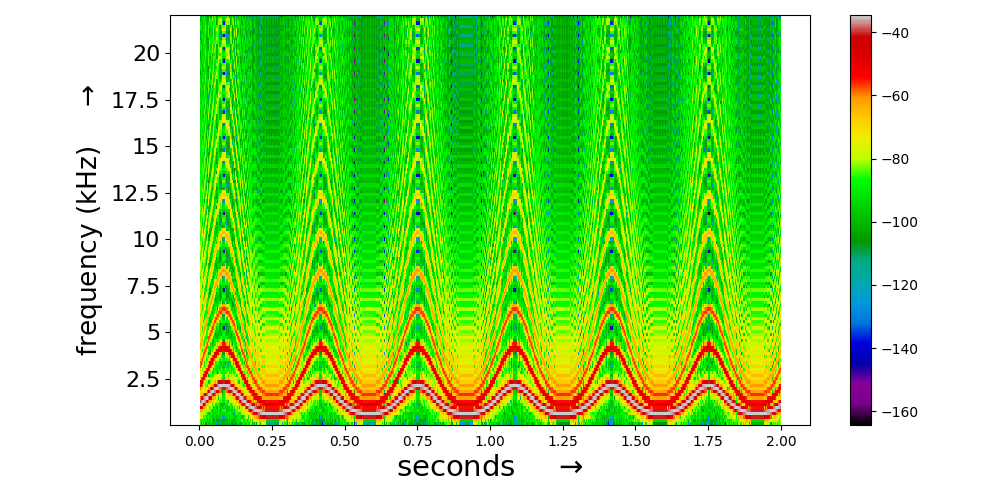
\includegraphics[width=\columnwidth]{figures/vibrato_}
     \caption{Spectrogram of a sound with a sinusoidal vibrato of $3Hz$ and one octave of depth in a $1000Hz$ sawtooth wave ($f_s=44.1kHz$). The color bar is in decibels.}
         \label{fig:vibrato}
\end{figure}

For the proper realization of the vibrato, it is important to pay attention to both tables and sequences. Table $\widetilde{M}$ with length $\widetilde{\Lambda}_M$ and the sequence of indices $\gamma_i'$ make the sequence $t_i'$ which is the oscillatory pattern in the frequency while table $\widetilde{L}$ with length $\widetilde{\Lambda}$ and the sequence of indices $\gamma_i$ make $t_i$ which is the sound itself. Variables $\mu$ and $\nu$ quantify the vibrato intensity:
\begin{itemize}
    \item $\mu$ is a direct measure of how many Hertz are involved in the upper limit of the oscillation, while
    \item $\nu$ is the direct measure of how many semitones (or half steps) are involved in the oscillation ($2\nu$ is the number of semitones between the upper and lower peaks of the frequency oscillations of the sound $\{t_i\}$).
\end{itemize}

It is convenient to use $\nu=\log_{2}\frac{f+\mu}{f} $ in this case because the maximum frequency increase is not equivalent to the maximum frequency decrease.
The maximum semitone/pitch displacement is the invariant quantity
and is called 'vibrato depth'.
Most often, a vibrato depth is specified in semitones or cents (one cent $= \frac{1}{100}$ of a semitone).

Figure~\ref{fig:vibrato} is the spectrogram of an artificial vibrato in a note with $1000Hz$,
in which the pitch deviation reaches one octave above and one below.
Practically any waveform can be used to generate a sound and the vibrato oscillatory pattern, with virtually any oscillation frequency and pitch deviation.
Such oscillations with precise waveforms and arbitrary amplitudes are not possible in traditional music instruments, and thus it introduces novelty in the artistic possibilities.

Tremolo is similar: $f'$, $\gamma_i'$ and $t_i'$ remain the same.
The amplitude sequence to be multiplied by the original sequence $t_i$ is:

\begin{equation}\label{trA}
 a_i=10^{\frac{V_{dB}}{20}t_i' } = a_{\text{max}}^{t_i'}
\end{equation}
\noindent and, finally: 

\begin{equation}\label{trT}
\begin{split}
 T^{tr(f')}=\left \{ t_i^{tr(f')} \right \}_0^{\Lambda-1}=\{ t_i . a_i \}_0^{\Lambda-1}= \left \{t_i .10^{t_i' \frac{V_{dB}}{20}}    \right \}_0^{\Lambda-1}=\left\{t_i . a_{\text{max}}^{t_i'} \right\}_0^{\Lambda-1}
\end{split}
\end{equation}

\noindent where $V_{dB}$ is the oscillation depth in decibels and $a_{\text{max}}=10^{\frac{V_{dB}}{20}}$ is the maximum amplitude gain.
The measurement in decibels is suitable because the maximum increase in amplitude is not equivalent to the maximum decrease, while the difference in decibels is preserved.
Notice that the tremolo is applied to a preexisting sound and
thus the characteristics of the tremolo do not need to be accounted for
when synthesizing such sound (if it is synthesized)
in contrast with making a sound with a vibrato.

Figure~\ref{fig:tremolo} shows the amplitude of the sequences $\{a_i\}_0^{\Lambda-1}$ and $\{t_i'\}_0^{\Lambda-1}$ for three oscillations of a tremolo with a sawtooth waveform. The curvature is due to the logarithmic progression of the intensity. The tremolo frequency is $1.5Hz$ if $f_s=44.1kHz$ because $\text{duration} = \frac{i_{\text{max}}=82000}{f_s}= 2s \; \Rightarrow \; \frac{3\text{oscillations}}{2s}=1.5$ oscillations per second.

The musical piece \emph{Shakes and Wiggles} explores these possibilities given by tremolos and vibratos,
both used in conjunction and independently (tremolos and vibratos occur many times together in a conventional music instrument),
with different frequencies $f'$, depths ($\nu$ and $V_{dB}$),
and progressive variations of parameters.
Aiming at a qualitative appreciation,
the piece also develops a comparison between vibratos and tremolos in logarithmic and linear scales.~\cite{MASSA}

\begin{figure*}
     \centering
         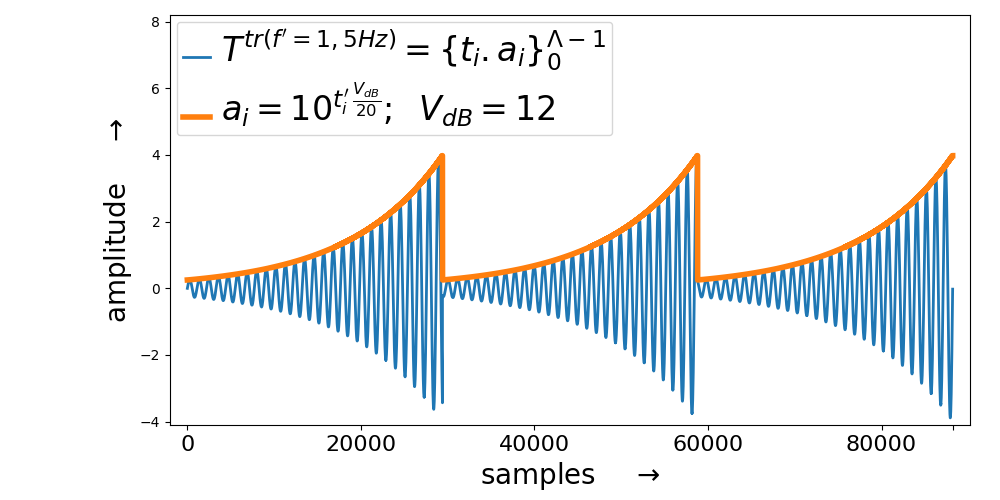
\includegraphics[width=\textwidth]{figures/tremolo_}
     \caption{Tremolo with a depth of $V_{dB}=12dB$, with a sawtooth waveform as its oscillatory pattern, with $f'=1.5Hz$ in a sine of $f=40Hz$ ($f_s=44.1kHz$).}
         \label{fig:tremolo}
\end{figure*}

The proximity of $f'$ to $20Hz$ generates roughness in both tremolos and vibratos. This roughness is largely appreciated both in traditional classical music and current electronic music, especially in the \emph{Dubstep} genre. Roughness is also generated by spectral content that produces beating~\cite{Porres,porres2009}. The sequence \emph{Bela Rugosi} explores this roughness threshold with concomitant tremolos and vibratos at the same voice, with different intensities and waveforms.~\cite{MASSA}

As the frequency increases further, these oscillations no longer remain noticeable individually.
In this case, the oscillations become audible as pitch.
Then, $f'$,
the depths ($\nu$ and $V_{dB}$),
and the waveform together change the audible spectrum of original sound $T$ in different ways for tremolos and vibratos. They are called AM (\emph{Amplitude Modulation}) and FM (\emph{Frequency Modulation}) synthesis,
respectively. These techniques are well known, with applications in
synthesizers like \emph{Yamaha DX7}, and even with applications outside music, as in telecommunications for data transfer by means of electromagnetic waves (e.g.\ AM and FM radios).

For musical goals, it is possible to understand FM based on the
case of sines and, when other waveforms are employed, to consider the signals by their respective Fourier components (i.e.\ sines as well).
The FM synthesis performed with a sinusoidal vibrato of frequency $f'$ and depth $\mu$ in a sinusoidal sound $T$ with frequency $f$ generates bands centered around $f$ and far from each other by $f'$:

\begin{equation}\label{eq:fmEsp}
\begin{split}
\{t_i'\} & = \left \{ \cos \left [f . 2 \pi \frac{i}{f_s-1} + \mu . sen \left ( f' . 2 \pi \frac{i}{ f_s -1 } \right ) \right ] \right \} = \\
 & = \left \{ \sum_{k=-\infty}^{+\infty} J_k(\mu) \cos \left [ f . 2 \pi \frac{i}{f_s-1} + k . f' . 2 \pi \frac{i}{f_s-1} \right ]  \right \} = \\
 & = \left \{ \sum_{k=-\infty}^{+\infty} J_k(\mu) \cos \left [ (f+k.f') . 2 \pi \frac{i}{f_s-1} \right ]  \right \}
\end{split}
\end{equation}

\noindent where

\begin{equation}\label{eq:Bessel}
J_k(\mu) = \frac{2}{\pi} \int_0^{\frac{\pi}{2}}\left [ cos \left (\overline{k}\;\frac{\pi}{2} + \mu . \sin w \right ) . cos \left ( \overline{k}\;\frac{\pi}{2} + k . w \right ) \right ] dw \;,\; \overline{k} = k \% 2 \;,\; k \in \mathbb{N}
\end{equation}

\noindent is the Bessel function~\cite{BesselCCRMA,JOSFM} and specifies the amplitude of each component in an FM synthesis.

In these equations, the frequency variation introduced by $\{t_i'\}$ does not follow the geometric progression that yields linear pitch variation, but reflects Equation~\ref{freqLinear}.
The result of using Equations~\ref{vbrF} for FM is described in the Appendix D of~\cite{dissertacao}, where the spectral content of the FM synthesis is calculated for oscillations in the logarithmic scale. In fact, the simple and attractive FM behavior is usually observed with linear oscillations, such as in Equation~\ref{eq:fmEsp}, which yield less strident and less noisy sounds.

For the amplitude modulation (AM):

\begin{equation}\label{eq:specAM}
\begin{split}
\{t_i'\}_0^{\Lambda-1} =\{(1+a_i) . t_i\}_0^{\Lambda-1} = \left \{ \left [ 1+M.\sin \left ( f'.2\pi\frac{i}{f_s -1} \right ) \right] .P .\sin \left ( f.2\pi\frac{i}{f_s -1} \right ) \right \}_0^{\Lambda-1} = \\ 
                        =  \left\{P.\sin \left( f.2\pi\frac{i}{f_s -1}  \right ) +  \frac{P.M}{2} \left [ \sin \left( (f-f').2\pi\frac{i}{f_s -1}  \right )  + \sin \left( (f+f').2\pi\frac{i}{f_s -1}  \right ) \right ] \right \}_0^{\Lambda-1}
\end{split}
\end{equation}

% \newcommand{\OneColEqu}[1]{%
% \end{multicols}%
% \begin{twocolequfloat}%
% \begin{equation}
% \{t_i'\}_0^{\Lambda-1} =\{(1+a_i) . t_i\}_0^{\Lambda-1} = \left \{ \left [ 1+M.\sin \left ( f'.2\pi\frac{i}{f_s -1} \right ) \right] .P .\sin \left ( f.2\pi\frac{i}{f_s -1} \right ) \right \}_0^{\Lambda-1} = \\ 
%                         =  \left\{P.\sin \left( f.2\pi\frac{i}{f_s -1}  \right ) +  \frac{P.M}{2} \left [ \sin \left( (f-f').2\pi\frac{i}{f_s -1}  \right )  + \sin \left( (f+f').2\pi\frac{i}{f_s -1}  \right ) \right ] \right \}_0^{\Lambda-1}
% \end{equation}
% \end{twocolequfloat}%
% \begin{multicols}{2}%
% }

The resulting sound is the original one together with the
reproduction of its spectral content below and above with a displacement of $f'$.
Again, this is achieved by variations in the linear scale (of the amplitude).
The spectrum of an AM performed with oscillations in the logarithmic amplitude scale is described in Appendix D of~\cite{dissertacao}.
The sequence $T$, with frequency $f$, called `carrier', is modulated by
$f'$, called 'modulator'. In FM and AM jargon, $\mu$ and
$a_{max}=10^{\frac{V_{dB}}{20}}$ are `modulation indexes'.
The following equations are defined for the oscillatory pattern of the modulator sequence $\{t_i'\}$:

\begin{equation}\label{fmGammaAux}
\gamma_i'=\left \lfloor i f' \frac{\widetilde{\Lambda}_M}{f_s} \right \rfloor
\end{equation}

\begin{equation}\label{fmAux}
t_i'=\widetilde{m}_{\gamma_i' \;\% \widetilde{\Lambda}_M}
\end{equation}

In FM, the modulator $\{t_i'\}$ is applied to the carrier $\{t_i\}$ by:

\begin{equation}\label{fmF}
f_i=f + \mu . t_i'
\end{equation}

\begin{equation}\label{fmGamma}
\Delta_{\gamma_i}=f_i\frac{\widetilde{\Lambda}}{f_s} \quad \Rightarrow \quad \gamma_i = \left \lfloor \sum_{j=0}^{i} f_j \frac{\widetilde{\Lambda}}{f_s} \right \rfloor = \left \lfloor \sum_{j=0}^{i} \frac{\widetilde{\Lambda}}{f_s}(f+\mu . t_j') \right\rfloor
\end{equation}

\begin{equation}\label{fmT}
T^{f,\, FM(f',\,\mu)}=\left\{ t_i^{f,\,FM(f',\,\mu)} \right\}_0^{\Lambda-1}=\left\{\,\widetilde{l}_{\gamma_i \%\; \widetilde{\Lambda} } \,\right\}_0^{\Lambda-1}
\end{equation}


\noindent where $\widetilde{l}$ is the waveform period with a length of $\widetilde{\Lambda}$ samples, used for the carrier signal.

To perform AM, the signal $\{t_i\}$ needs to be modulated with $\{t_i'\}$ using the following equations:

\begin{equation}\label{amA}
a_i=1 + \alpha . t_i'
\end{equation}

\begin{equation}\label{amT}
T^{f,\,AM(f',\,\alpha)}=\left\{ t_i^{f,\,AM(f',\,\alpha)} \right\}_0^{\Lambda-1}=\{ t_i . a_i \}_0^{\Lambda-1}= \{t_i . (1 + \alpha . t_i')    \}_0^{\Lambda-1}
\end{equation}

\subsection{Musical usages}\label{subsec:mus2}
At this point the musical possibilities are very wide.
Sonic characteristics, like pitch (given by frequency),
timbre (achieved by waveforms, filters and noise) and loudness (manipulated by intensity)
can be considered in an absolute form or varied throughout the duration of a sound
or a musical piece.
The following musical usages encompass a collection of possibilities with the purpose of exemplifying types of sonic manipulations that result in musical material.
Some of them are discussed more deeply in the next section.

\subsubsection{Relations between characteristics}
This is a widespread procedure used to obtain musically attractive and coherent excerpts.
A possibility is to establish relations between parameters of
tremolos and vibratos, and of the basic note like frequency.
Let a vibrato frequency be proportional
to note pitch, or a tremolo depth be inversely proportional to
pitch. Therefore, with Equations~\ref{vbrGamma},~\ref{vbrF} and~\ref{trA}:

\begin{equation}\label{eq:vinculos}
\begin{split}
f^{vbr} = f^{tr} & = func_a(f) \\
\nu & = func_b(f) \\
V_{dB} & = func_c(f)
\end{split}
\end{equation}

\noindent with $f^{vbr}$ and $f^{tr}$ as $f'$ in the referenced equations.
 $\nu$ and $V_{dB}$ are the respective depth values of vibrato and
tremolo. Functions $func_a$, $func_b$ and $func_c$ are arbitrary and dependent on musical intentions.
The music piece \emph{Bonds} explores such bonds and exhibits variations in the waveforms with the purpose of building a \emph{musical
language} (details in a Supporting Information document of this article~\cite{massNotesInMusic}).~\cite{MASSA}

\subsubsection{Convolution for rhythm and meter}
A musical pulse - such as specified by a BPM
tempo - can be implied by an impulse at the start of each beat: the convolution with an impulse shifts the sound to impulse position, as stated in Section~\ref{subsec:conv}. For example, two impulses equally spaced build a binary division of the
pulse.
Two signals, one with 2 impulses and the other with 3 impulses, both equally spaced in the pulse duration, yield a pulse
maintenance with a rhythm which eases both binary or ternary
divisions.
This is found in many ethnic and traditional musical styles~\cite{Gramani}.
The absolute values of the impulses entail
proportions among the amplitudes of the sonic re-incidences.
The use of convolution with impulses in this context is explored in the music piece \emph{Little train of impulsive hillbillies}.
These procedures also encompass
the creation of `sound amalgams' based on granular synthesis; see Figure~\ref*{fig:pulsoSubAgl} of the Supporting Information~\cite{massNotesInMusic}.~\cite{MASSA}


\subsubsection{Moving source and receptor, Doppler effect}
According to the discussion in Section~\ref{subsec:spac},
when an audio source (or receptor) is moving,
the IID and ITD are constantly changing and
are ideally updated at each sample of the digital signal 
(if fast computational rendering is not at stake).
As given by basic theory,
the audio source speed $s_s$, with positive values if the source moves away from receptor,
and receptor speed $s_r$, positive when it gets closer to audio source (one might always use $s_r=0$ for musical purposes),
relates the frequency $f$ as perceived by the receiver
and the frequency $f_0$ emitted by:

\begin{equation}\label{eq:fDoppler}
    f=\left(\frac{s_{sound}+s_r}{s_{sound}+s_s}\right)f_0
\end{equation}

Using the coordinates as in Figure~\ref{fig:spac},
and Equation~\ref{eq:distOuvidos},
the speed $s_s$ can be found simply by $s_s = f_s(d_{i+1}-d_{i})$.
One should also use IID for the intensity progression of the sound,
and ITD to correctly start and end the sonic
sequences related to each ear.
The change in pitch is antisymmetric
upon the crossing of source with receptor:
the same semitones (or fraction of) that are added during the approach are decreased during the departure.
Moreover, the transition is abrupt if source and receptor intersect with zero distance, otherwise, there is a smooth progression.

% The musical piece \emph{Doppeleer} explores and exemplifies the musical use of the Doppler effect.~\cite{MASSA}

\subsubsection{Filters and noises}
With the use of filters, the possibilities are even wider.
Convolve a signal to have a reverberated version of it, to remove its noise, to distort or to handle
the audio aesthetically in many other ways. For example, sounds originated from an old television or telephone can be simulated with a band-pass filter, allowing only frequencies between $1kHz$ and $3kHz$. By rejecting the frequency of an electric oscillation (usually $50Hz$ or $60Hz$) and the harmonics, one can remove noises caused by audio devices connected to the power supply. A more musical application is to perform filtering in specific bands and to use those bands as an additional parameter to the notes.

Inspired by traditional music instruments, it is possible to apply a
time-dependent filter~\cite{Roederer}. Chaining such filters can be useful for performing complex and more accurate filtering routines. The musical piece \emph{Noisy band} explores filters and many kinds and noise synthesis.~\cite{MASSA}

A sound can be altered through different filtering processes and then mixed to create an effect known as \emph{chorus}. Based on what happens in a choir of singers, the sound is synthesized using small and potentially arbitrary modifications of parameters like center frequency, presence (or absence) of vibrato or tremolo and its characteristics, equalization, loudness, etc. As a final result, those versions of the original sound are mixed together (see Equation~\ref{eq:mixagem}).
The musical piece \emph{Children choir} implements a very simple chorus
and applies it to structures described in the next section.~\cite{MASSA}

\subsubsection{Reverberation}\label{subsubsec:reverb}
Using the same terms of Section~\ref{subsec:spac}, the
late reverberation can be achieved by a convolution with a section of pink, brown or black noise, with an exponential decay of amplitude along time. Delay lines can be added as a prefix to the noise
with the decay, and this accounts for both time parts of the reverberation: the early reflections and the late reverberation. Quality can be improved by varying the geometric trajectory and filtering by each surface where the wavefront reflected before reaching the ear in the first $100-200ms$ (mainly with a LP). The colored noise can be gradually introduced with a \emph{fade-in}: the initial moment given by direct
incidence of sound (i.e.\ without any reflection and given by ITD and IID), reaching its maximum at the beginning of the 'late
reverberation', when the geometric incidences loose their relevance to the statistical properties of the decaying noise.
As an example, consider $\Delta_1$ as the duration of the first reverberation section and 
$\Delta_R$ as the complete duration of the reverberation ($\Lambda_1=\Delta_1 f_s$, $\Lambda_R=\Delta_R
f_s$). Let $p_i$ be the probability of a sound to be repeated in the
$i$-th sample.
Following
Section~\ref{subsec:spac}, the sequence $R^1$ with the amplitudes of the
impulse response of the first period can be described as:

\begin{equation}\label{eq:p1rev}
\begin{split}
	R^1  =\left\{r_i^1\right\}_0^{\Lambda_1-1}\;,\; \text{where}\;\;
	r_i^1  =\left\{
        \begin{array}{l l}
            10^{\frac{V_{dB}}{20}\frac{i}{\Lambda_R-1}}\;  & \text{with probability}\quad p_i=\left(\frac{i}{\Lambda_1}\right)^2 \\
                                     0 \; & \text{with probability}\quad 1-p_i \\
        \end{array} \right.
\end{split}
\end{equation}

\noindent where $V_{dB}$ is the total decay in decibels, typically $-80dB$ or $-120dB$.
The sequence $R^2$ with the samples of the impulse response of the second period can be
obtained from a brown noise $N^b$ (or by a pink noise $N^p$) with an exponential amplitude decay of the waveform:

\begin{equation}\label{eq:p2rev}
    R^2=\left\{r_i^2\right\}_{\Lambda_1}^{\Lambda_R-1}=\left\{10^{\frac{V_{dB}}{20}\frac{i}{\Lambda_R-1}}\,.\,r_i^b\right\}_{\Lambda_1}^{\Lambda_R-1}
\end{equation}

Finally:

\begin{equation}\label{eq:rev}
	R=\left\{r_i\right\}_0^{\Lambda_R-1}\;,\; \text{where} \; r_i=\left\{
        \begin{array}{l l}
            r_i^1\;  & \text{if }\quad 0\leq i<\Lambda_1-1 \\
                                     r_i^2 \; & \text{if}\quad \Lambda_1 \leq i < \Lambda_R-1 \\
        \end{array} \right.
\end{equation}

A sound with an artificial reverberation can be achieved by a simple convolution of $R$ (called reverberation impulse response) with the sound sequence $T$, as described in Section~\ref{subsec:filtros}. Reverberation is well known for causing great interest in listeners and to provide sonorities that are more enjoyable. Furthermore, modifications in the reverberation consist in a common technique (almost a \textit{clich\'{e}}) to surprise and attract the listener.
% The musical piece \emph{Re-verb} explores reverberations in various settings.~\cite{MASSA}

\subsubsection{ADSR envelopes}
The variation of loudness along the duration of a sound is crucial to our timbre perception.
The intensity envelope known as ADSR (\emph{Attack-Decay-Sustain-Release}) has many implementations in both hardware and software synthesizers. A pioneering implementation can be found in the Hammond Novachord synthesizer of 1938 and some variants are mentioned below~\cite{ADSR}. The canonical ADSR envelope is characterized by 4 parameters: attack duration (time at which the sound reaches its maximum amplitude), decay duration (follows the attack immediately), level of sustained intensity (in which the intensity remains stable after the decay) and release duration (after sustained section, this is the duration needed for amplitude to reach zero or final value).
Note that the sustain duration is not specified because it is the difference between the total duration and the sum of the attack, decay and release durations.

\begin{figure}[htp!]
    \centering
        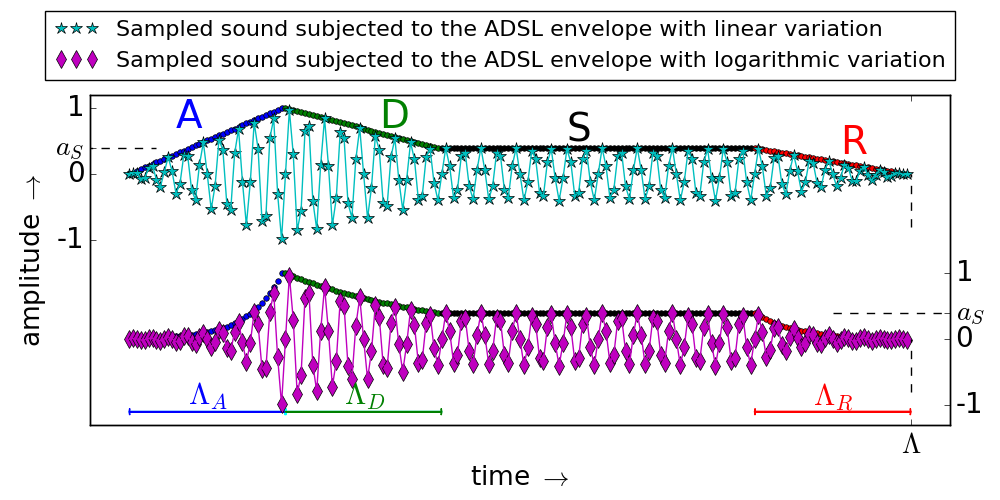
\includegraphics[width=\columnwidth]{figures/adsr_}
    \caption{An ADSR envelope (\emph{Attack, Decay, Sustain, Release}) applied to an arbitrary sound sequence. The linear variation of the amplitude is above, in blue. Below the amplitude variation is exponential.}
        \label{fig:adsr}
\end{figure}

The ADSR envelope with durations $\Delta_A$, $\Delta_D$ and $\Delta_R$, with total duration $\Delta$ and sustain level $a_S$, given as the fraction of the maximum amplitude, to be applied to any sound sequence $T=\{t_i\}$ (ideally also with duration $\Delta$), can be expressed as:

\begin{equation}\label{eq:adsr}
\begin{split}
\{a_i\}_0^{\Lambda_A-1}  = & \left\{\xi\left(\frac{1}{\xi}\right)^{\frac{i}{\Lambda_A-1}}\right\}_0^{\Lambda_A-1} \quad \text{ or }\\ = & \left\{\frac{i}{\Lambda_A-1}\right\}_0^{\Lambda_A}\\
\{a_i\}_{\Lambda_A}^{\Lambda_A+\Lambda_D-1} = & \left\{a_S^{\frac{i-\Lambda_A}{\Lambda_D-1}}  \right\}_{\Lambda_A}^{\Lambda_A+\Lambda_D-1} \quad \text{ or } \\ = &  \left\{1-(1-a_S)\frac{i-\Lambda_A}{\Lambda_D-1}\right\}_{\Lambda_A}^{\Lambda_A+\Lambda_D-1}\\
\{ a_i \}_{\Lambda_A+\Lambda_D}^{\Lambda-\Lambda_R-1} = & \left\{ a_S \right\}_{\Lambda_A+\Lambda_D}^{\Lambda-\Lambda_R-1} \\
\{ a_i \}_{\Lambda-\Lambda_R}^{\Lambda-1}  = & \left\{ a_S\left(\frac{\xi}{a_S} \right)^{\frac{i-(\Lambda-\Lambda_R)}{\Lambda_R-1}} \right\}_{\Lambda-\Lambda_R}^{\Lambda-1} \quad \text{ or } \\ = &  \left\{ a_S - a_S\frac{i+\Lambda_R-\Lambda}{\Lambda_R-1}\right\}_{\Lambda-\Lambda_R}^{\Lambda-1} 
\end{split}
\end{equation}

\noindent with $\Lambda_X=\lfloor \Delta_X . f_s \rfloor\;\;\forall\;\; X \; \in
(A,D,R\;)$ and $\xi$ being a small value that provides a satisfactory \emph{fade in} and \emph{fade out}, e.g.\ $\xi=10^{\frac{-80}{20}}=10^{-4}\;$.
The lower the $\xi$, the slower the \emph{fade}, similar to the $\alpha$ illustrated in Figure~\ref{fig:transicao}.
One might also use a linear or quartic ($x^4$) fade at the beginning of the attack and the end of the release
sections to reach zero amplitude (exponential fades never reach zero).
Schematically, Figure~\ref{fig:adsr} shows the ADSR envelope in a classical implementation that supports many variations.
For example, between attack and decay it is possible to add an extra section where the maximum amplitude remains for more than a peak.
Another common example is the use of more elaborated envelopes for attack or decay.
The music piece \emph{ADa and SaRa} explores many configurations of the ADSR envelope.~\cite{MASSA}

\begin{equation}\label{eq:adsrApl}
\left\{t_i^{ADSR}\right\}_0^{\Lambda-1} =\{t_i . a_i\}_0^{\Lambda-1}
\end{equation}

\section{Conclusions and further developments}
\label{cap:conclusao}
In our understanding,
this article is effective in relating musical elements to digital audio.
We aimed at achieving a concise presentation of the subject because it involves many knowledge fields, and therefore can very easily blast into thousands of pages.
Some readers might benefit from the text alone, but the \emph{scripts} in the \massa\ toolbox, where all the equations and concepts are directly and simply implemented as software (in Python),
are very helpful for one to achieve elaborated implementations and deeper understandings.
The scripts include routines that render musical pieces to illustrate the concepts in practical contexts.
This is valuable since art (music) can involve many non-trivial processes and is often deeply glamorized, which results in a nearly unmanageable terrain for a newcomer.
Moreover, this didactic report and the supplied open source scripts should facilitate the use of the framework.
One of the Supporting Information documents~\cite{massListings} holds listings of sections, equations, figures, tables, scripts and other documents.
Another Supporting Information document~\cite{massCode} holds a PDF presentation of the code related to each section
because many readers might not find it easy to browse source code files.
Most importantly, an extension of the preceding sections to encompass the organization of notes in music, as managed by canonical music theory, is yet in another Supporting Information document~\cite{massNotesInMusic}.

The possibilities provided by this exposition pour from both the organization of knowledge and the ability to achieve sounds which are extremely true to the models.
For example, one can produce noises with an arbitrary resolution of the spectrum and a musical note can be synthesized with the parameters (e.g. of a vibrato) updated sample-by-sample.
Furthermore, software for synthesis and processing of sounds for musical purposes
by standard restricts the bit depth to 16 or 24.
This is achievable in this framework but by standard Python uses more bits per floating point number.
These ``higher fidelity'' characteristics can be crucial
e.g. for psychoacoustic experiments or to generate high quality musical sounds or pieces.
Simply put, it is compelling
for many scientific and artistic purposes.
The didactic potential of the framework is evident when noticed that:
\begin{itemize}
	\item the integrals and derivatives, ubiquitous in continuous signal processing,
are all replaced, in discrete signals, by summations,
which are more intuitive and does not require fluency in calculus.
	\item The equations and concepts are implemented in a simple and straightforward manner as software which can be easily assembled and inspected.
\end{itemize}
\noindent In fact, this framework was used in a number of contexts, including courses, software implementations and for making music~\cite{vimeoLM,vivace,dissertacao}.
As far as the authors know, such detailed analytical descriptions have not been covered before in the literature, such as testified in the literature review (Appendix G of~\cite{dissertacao}, where books, articles and open software are related to this framework).

The free software license, and online availability of the content,
facilitate collaborations and the generation of sub-products in a co-authorship fashion,
new implementations and development of musical pieces.
The scripts can be divided in three groups: implementation of all the equations and topics of music theory covered here; routines for rendering musical pieces that illustrate the concepts; scripts that render the figures of this article and the article itself.

This framework favored the formation of interest groups in topics such as musical creativity and computer music.
In particular, the project \url{labMacambira.sourceforge.net} groups Brazilian and foreign co-workers
in diverse areas that range from digital direct democracy and georeferencing to art and education.
This was only possible because of the usefulness of audiovisual abilities in many contexts, in particular because of the knowledge and mastery condensed in the \massa\ framework.\footnote{There are more than 700 videos, written documents,
 original software applications and contributions in well-known software (such as Firefox, Scilab, LibreOffice, GEM/Puredata, to name just a few)~\cite{siteLM,wikiLM,vimeoLM}.
Some of these efforts are available online~\cite{dissertacao}.
It is evident that all these contributions are a consequence of more that just \massa, but it is also evident to the authors that \massa\ had a primary role in converging interests and attracting collaborators.}

Future work might include application of these results in artificial intelligence
for the generation of attractive artistic materials. Some psychoacoustic effects were detected,
which need validation and should be reported, specially with~\cite{quadrosSonoros}.\footnote{The sonic portraits where sent to a public mailing list~\cite{metaLista} and the fifth piece was reported by some individuals to induce a state in which noises from the own tongue, teeth and jaw of the individual echoed for some seconds (the GMANE archives with the descriptions of the effect by listeners in the public email list is unfortunately offline at the moment).} Other foreseen advances
are: enhancement of the Python package written using \massa~\cite{music}, a JavaScript version of the toolbox, better hypermedia deliverables of this framework, user guides
for different goals (e.g. musical composition, psychophysic experiments, sound synthesis, education), creation
of more musical pieces, open experiments to be studied with EEG recordings, a linked data representation
of the knowledge in \massa\ through SKOS and OWL to tackle the issues exposed in Section~\ref{sec:disc},
data sonification routines, and further analytical specification of musical
elements in the discrete-time representation of sound as feedback is received from the community.

\begin{acks}
    This work was supported by Capes, CNPq and FAPESP (projects 2013/14262-7 and 2017/05838-3).
\end{acks}

% Bibliography
\bibliographystyle{ACM-Reference-Format}
% \bibliography{sample-bibliography}
\bibliography{./article2}
